\documentclass[11pt]{article}
\usepackage[T1]{fontenc}
\usepackage[utf8]{inputenc}
\usepackage{lmodern}
\usepackage[margin=1.05in]{geometry}
\usepackage{amsmath,amssymb,amsthm,mathtools}
\numberwithin{equation}{section}
\usepackage{microtype}
\usepackage{enumitem,booktabs,array}
\usepackage{needspace,etoolbox}
\usepackage{tikz}
\usetikzlibrary{arrows.meta,positioning,calc,patterns}
\usepackage{xcolor}
\usepackage[hypertexnames=false,colorlinks=true,linkcolor=blue!45!black,citecolor=green!35!black,urlcolor=blue!45!black]{hyperref}
\hypersetup{pdftitle={The Critical Spin Field of the Planar XY Model},pdfauthor={OpenAI}}
\newtheorem{theorem}{Theorem}[section]
\newtheorem{lemma}[theorem]{Lemma}
\newtheorem{proposition}[theorem]{Proposition}
\newtheorem{corollary}[theorem]{Corollary}
\theoremstyle{definition}
\newtheorem{definition}[theorem]{Definition}
\theoremstyle{remark}
\newtheorem{remark}[theorem]{Remark}
\BeforeBeginEnvironment{theorem}{\Needspace{6\baselineskip}}
\BeforeBeginEnvironment{lemma}{\Needspace{6\baselineskip}}
\BeforeBeginEnvironment{proposition}{\Needspace{6\baselineskip}}
\BeforeBeginEnvironment{corollary}{\Needspace{6\baselineskip}}
\BeforeBeginEnvironment{definition}{\Needspace{6\baselineskip}}
\preto\subsection{\Needspace{9\baselineskip}}
\newcommand{\R}{\mathbb R}
\newcommand{\Z}{\mathbb Z}
\newcommand{\C}{\mathbb C}
\newcommand{\N}{\mathbb N}
\newcommand{\E}{\mathbb E}
\newcommand{\Pbb}{\mathbb P}
\DeclareMathOperator{\Var}{Var}
\DeclareMathOperator{\Cov}{Cov}
\DeclareMathOperator{\supp}{supp}
\DeclareMathOperator{\diam}{diam}
\DeclareMathOperator{\dist}{dist}
\DeclareMathOperator{\Tr}{Tr}
\setlist{topsep=4pt,itemsep=3pt,parsep=0pt}
\setlength{\emergencystretch}{1.5em}
\clubpenalty=10000
\widowpenalty=10000
\displaywidowpenalty=10000
\title{The Critical Spin Field of the Planar XY Model}
\author{OpenAI}
\date{October 5, 2026}
\begin{document}
\maketitle
\begin{abstract}
Using the companion critical Bessel-height and pin-limit theorems, we
prove that at the mass-defined critical inverse temperature of the
nearest-neighbor XY model on the square lattice, the spin field on a
square with boundary angles fixed to zero converges along the full
sequence to the full-variance imaginary exponential of a zero-Dirichlet
Gaussian free field with stiffness \(2/\pi\). The normalization uses
the exact center magnetization and the lattice Green-function factor.
Convergence holds in law in \(H^{-3}_{\mathrm{loc}}((-1,1)^2)\);
all mixed moments and joint laws of fields smeared against smooth
compactly supported test functions in \((-1,1)^2\) converge as well.
\end{abstract}
\tableofcontents
\section{Introduction}\label{sec:intro}

The two-dimensional XY model has a massless phase without ordinary
long-range order. Its expected large-scale description is Gaussian, but
the spin is an exponential of an angular variable, not the angular
variable itself. Identifying a height-field limit therefore does not by
itself identify the spin field. At criticality a further difficulty is
that a scale-dependent scalar factor may survive between the microscopic
spin and its continuum normalization.

We prove a critical spin-field limit on a square with fixed boundary
spins. The scalar normalization is the actual magnetization at the
center of that square. This choice cancels the microscopic amplitude
without assuming a power law, a logarithmic correction, or the existence
of an asymptotic amplitude. The remaining spatial normalization is fixed
by the lattice Green function.

\subsection{The physical critical parameter}

We first specify the critical inverse temperature using an infinite-volume
quantity, independently of the field limit. For \(R\in\N\), let
\[
 \Lambda_R=[-R,R]^2\cap\Z^2,\qquad
 E_R=\{\{x,y\}\subset\Lambda_R:|x-y|=1\}.
\]
Every unordered edge occurs once. At inverse temperature \(b>0\), the
free-box law is
\begin{equation}\label{eq:free-spin-law}
 \frac1{Z_{R,b}}
 \exp\!\left\{b\sum_{\{x,y\}\in E_R}\cos(\theta_x-\theta_y)\right\}
 \prod_{x\in\Lambda_R}\frac{d\theta_x}{2\pi},
 \qquad \theta_x\in\R/(2\pi\Z).
\end{equation}
There are no exterior edges or fixed spins in this definition. Write
\begin{equation}\label{eq:critical-parameter}
 \begin{split}
 C_b(r)&=\lim_{\substack{R\to\infty\\R\ge r}}
       \E_{R,b}\cos(\theta_0-\theta_{re_1}),\qquad e_1=(1,0),\\
 m(b)&=\lim_{r\to\infty}-\frac1r\log C_b(r),\qquad
 b_c=\inf\{b>0:m(b)=0\}.
 \end{split}
\end{equation}
The free-box correlation and mass limits exist,
\(0<b_c<\infty\), and \(m(b_c)=0\). These are the usual
phase-transition facts for the cosine convention
\eqref{eq:free-spin-law}; see \cite[Theorem 1]{vEL} and the
normalization comparison in \cite[Proposition~1.2]{C}. No critical exponent is included
in the definition of \(b_c\).

\subsection{The normalized spin field}

For each integer \(n\ge1\), set
\[
 D=(-1,1)^2,\qquad D_n=[-1,1]^2\cap n^{-1}\Z^2,
 \qquad D_n^\circ=D_n\cap D.
\]
Let \(E_n\) contain all unordered nearest-neighbor pairs in \(D_n\).
Set \(\theta_x=0\) on \(D_n\setminus D_n^\circ\), and integrate only
the interior angles in the probability law
\begin{equation}\label{eq:pinned-spin-law}
 \frac1{Z_n^0}
 \exp\!\left\{b_c\sum_{\{x,y\}\in E_n}
                         \cos(\theta_x-\theta_y)\right\}
 \prod_{x\in D_n^\circ}\frac{d\theta_x}{2\pi}.
\end{equation}
Its expectation is denoted by \(\E_n^0\). In particular edges incident
to the fixed boundary are retained. Define
\begin{equation}\label{eq:center-magnetization}
 a_n=\E_n^0\cos\theta_0=\E_n^0e^{i\theta_0}>0.
\end{equation}
Angle reflection proves the equality, and the positive Fourier-current
expansion proves strict positivity. Thus \(a_n\) is a specified
observable of \eqref{eq:pinned-spin-law}, not a sequence chosen to fit
a limit.

On functions zero at the boundary let
\[
 (L_nu)(x)=\sum_{\substack{y\in D_n\\|x-y|=1/n}}
                   (u(x)-u(y)),\qquad G_n=L_n^{-1}.
\]
The Laplacian is unscaled: it contains no factor \(n^2\).
Put \(K_*=2/\pi\), and define the complex random distribution
\begin{equation}\label{eq:spin-field}
 S_n=\frac1{n^2}\sum_{x\in D_n^\circ}
 a_n^{-1}\exp\!\left\{\frac{G_n(x,x)-G_n(0,0)}{2K_*}\right\}
 e^{i\theta_x}\delta_x,
 \qquad \delta_x(f)=f(x).
\end{equation}
The center factor and the Green correction in this definition are
the same for every test function and every correlation order.

Let \(\Phi_D\) be the real zero-Dirichlet Gaussian free field with
covariance \((-\Delta_D)^{-1}\). Its kernel has the convention
\[
 G_D(z,w)=\frac1{2\pi}\log\frac1{|z-w|}+R_D(z,w),
\]
where \(R_D\) is smooth across the interior diagonal. For circle
averages \(\Phi_{D,\epsilon}\), taken where the circles lie in \(D\),
let
\begin{equation}\label{eq:target-field}
 V_*=\lim_{\epsilon\downarrow0}
 \exp\!\left\{\frac{i\Phi_{D,\epsilon}}{\sqrt{K_*}}
       +\frac{\E\Phi_{D,\epsilon}^2}{2K_*}\right\}.
\end{equation}
The limit is understood as a complex random distribution tested
against compactly supported smooth functions. This is the
full-variance imaginary Gaussian chaos: its counterterm uses the
entire variance, including its finite spatial part.
In this convention
\[
 \E V_*(f)=\int_D f(z)\,dz,\qquad
 \E\bigl[V_*(z)\overline{V_*(w)}\bigr]
       =\exp\{G_D(z,w)/K_*\},
\]
where the second expression denotes the off-diagonal moment kernel.
Its singularity has exponent \(1/4\). Existence and the precise
mixed-moment interpretation are recalled in
Lemma~\ref{fields:circle-chaos}; see also \cite{JSW2020,B}.

\begin{theorem}\label{thm:main}
For the fixed-boundary critical XY law \eqref{eq:pinned-spin-law},
the distributions \(S_n\) in \eqref{eq:spin-field} converge in law
along the full sequence \(n\to\infty\) to \(V_*\) in
\(H^{-3}_{\mathrm{loc}}(D)\).
Moreover, for every \(k\ge1\), every
\(f_1,\ldots,f_k\in C_c^\infty(D;\C)\), and every collection of
nonnegative integers \(p_1,q_1,\ldots,p_k,q_k\),
\begin{equation}\label{eq:main-moment-convergence}
 \E_n^0\prod_{j=1}^k
       S_n(f_j)^{p_j}\overline{S_n(f_j)}^{\,q_j}
 \longrightarrow
 \E\prod_{j=1}^k
       V_*(f_j)^{p_j}\overline{V_*(f_j)}^{\,q_j}.
\end{equation}
The joint laws of these complex smeared fields converge as well.
\end{theorem}

Here \(H^{-3}_{\mathrm{loc}}(D)\) consists of distributions \(T\)
such that \(\chi T\), extended by zero, belongs to
\(H^{-3}(\R^2)\) for every \(\chi\in C_c^\infty(D)\), with the
usual local topology. The theorem includes nonneutral moments:
there is no requirement that the total number of fields equal
the total number of conjugate fields.

The critical input is the Bessel-height coefficient and the height
and pin limit theorems of \cite{C}. Their exact statements and
conventions are recorded in Section~\ref{sec:heights}; the critical
coefficient there is \(a(b_c)=8\pi\), giving
\(K_*=a(b_c)/(4\pi^2)\). We also use the finite comparisons and field
lemmas identified in \cite{B}. We do not deduce the result by
continuing a low-temperature spin theorem to \(b_c\).
Nor does Theorem~\ref{thm:main} assert an asymptotic formula for
\(a_n\), or by itself transfer the result to the free-boundary
infinite-volume correlation. Such a transfer would require
additional amplitude and boundary-to-bulk information.

\subsection{Historical context and related work}

The distinction between absence of magnetization and slowly decaying
correlations is central to the two-dimensional XY model. Mermin and
Wagner~\cite{MW} established the low-dimensional obstruction to
conventional order for isotropic Heisenberg systems. For classical
planar spins, McBryan and Spencer~\cite{MS} obtained quantitative
power-law upper bounds on correlations. Berezinskii~\cite{Berezinskii}
developed the algebraic low-temperature picture and argued for a
phase transition. Kosterlitz and Thouless~\cite{BKT1973} proposed
the transition mechanism through the behavior of topological defects.
The ensuing renormalization-group theory predicts
the critical exponent \(1/4\) and renormalized stiffness
\(2/\pi\)~\cite{Kosterlitz1974,NK}.

Fr\"ohlich and Spencer~\cite{FS} proved a low-temperature phase with
power-law lower bounds for the rotator model and related systems.
Van Engelenburg and Lis~\cite[Theorem 1]{vEL} established a sharp
exponential-versus-polynomial dichotomy for free infinite-volume XY
correlations, including a polynomial lower bound at the threshold.
Lammers~\cite[Theorem 1]{Lammers2023} related the spin and dual-height
correlation lengths and identified the coincidence of the XY
transition with dual-height delocalization. These results identify
the physical threshold in Equation~\eqref{eq:critical-parameter};
they do not supply the critical spin-field limit.

Gaussian descriptions of angular fluctuations also have rigorous
precedents. Newman and Wu~\cite[Theorem 2]{NewmanWu2018} proved
Gaussian limits for angular-gradient observables in a joint
zero-temperature and continuum regime. The companion
\cite[Theorem 7.6]{B} treats the exponential spin field at sufficiently
low fixed temperature. The critical coefficient and fixed-geometry
Bessel-height inputs used here come instead from
\cite[Section 6 and Theorems 2.4, 3.1, 3.2]{C}.
Our task is to pass from these critical inputs to the spin field,
retaining the actual center magnetization as normalizer and treating
all signed correlations, including nonneutral ones.

The proof begins with integer-current and planar-height
duality~\cite[Section 2]{vEL}. The finite comparisons descend from
the lattice-Gaussian inequalities of Regev and
Stephens-Davidowitz~\cite{RSD}, in their Bessel-height form
in~\cite{C}. The target belongs to the theory of imaginary Gaussian
multiplicative chaos developed by Junnila, Saksman and
Webb~\cite{JSW2020}. To pass from correlations to field laws and
moments, we use the Lee--Yang theorem for planar
rotators~\cite{DunlopNewman1975} and its moment-generating-function
inequalities~\cite{Newman1975}, in the finite-volume formulation
of Newman and Wu~\cite{NewmanWu2019}. The sharp comparison for holes
of positive radius and the control of arbitrarily many annular
interfaces are developed below.

\subsection{Proof strategy}

Fourier expansion turns a product of spins into a ratio of height
partition functions. A spin insertion prescribes an integral winding
of the dual height around its location. We call a height law with
such prescribed windings a magnetic sector. Fixed spin boundary
conditions give free dual heights, modulo one common integer
translation.

The height limit does not directly determine a magnetic-sector
ratio when a puncture has the size of one lattice spacing. We first
keep every puncture at a positive macroscopic radius. For such
fixed domains, Section~\ref{sec:sectors} proves the sharp Gaussian
variational formula. Its upper bound uses divergence-free tests.
Its lower bound introduces quadratic penalties on box averages,
uses separated-pin estimates to compare pieces, and refines the
observation cells to recover the Dirichlet energy. All height limits
occur at fixed geometry.

To return to microscopic punctures, we surround each spin insertion
by a sequence of annuli. At an interface, the gluing kernel is the
partition-function factor for restoring the deleted bonds, conditional
on all height differences in a separating band. The integer constant
between two pieces is still summed. This relative-data convention
is essential both for exact factorization and for the treatment of
the free constant mode.

Sections~\ref{sec:annuli} and~\ref{sec:kernels} give two different
controls on these kernels. After division by their centered
zero-data value, they lie between zero and one for every datum.
Their average loss from one is small on long, approximately circular
annuli, including in a unit magnetic sector. These estimates are
not multiplied into an error proportional to the number of scales.
Instead, a contraction on mean-zero functions shows that an
arbitrary fixed microscopic core eventually produces a last-band
density bounded by two relative to the free annulus law. The core
may have an arbitrarily poor initial gluing factor; positivity is
enough.

We then attach all the annular sequences to one exterior region.
The exterior has positive-radius holes and is governed by the
variational formula already proved. The entire microscopic
contribution is the same for every unit insertion and for the
single insertion defining \(a_n\). Subtracting the corresponding
logarithms cancels that contribution exactly. Section~\ref{sec:correlations}
computes the remaining Green-function interaction and proves
uniform convergence on separated compact configurations.

The final step needs more than separated correlations. A weaker,
integrable two-point bound controls collisions uniformly in \(n\).
Together with positivity and the Lee--Yang moment estimate, it
removes every collision region from every mixed moment, without
requiring a sharp pointwise bound for higher correlations.
Section~\ref{sec:fields} then identifies the moments, proves
moment determinacy, and obtains local Sobolev tightness.

The sharp fixed-hole comparison and the positive-kernel stability
argument are the transferable parts of the proof. They separate
fixed-geometry Gaussian information from the microscopic
normalization, and use averaged control of conditional data where
a uniform conditional limit is unavailable.

\section{Free heights and finite comparisons}\label{sec:heights}

The fixed spin boundary becomes a free boundary after duality. We first
establish this correspondence, including nonneutral charges, and then
record the height limits that we use from \cite{C}. The finite comparisons
must keep track of independent additive constants and prescribed data
consisting only of height differences. We spell out how the cited
inequalities apply with these conventions.

\subsection{Partition sums and fixed-spin duality}

Choose one orientation of every edge of a finite nearest-neighbor graph
\(G=(V,E)\), and write \(\nabla_eh=h_y-h_x\) for \(e=(x,y)\).
We call its vertices and edges primary, to distinguish them from the
auxiliary subdivisions used below.
An \emph{integral connection} is an antisymmetric edge function
\(\alpha\) with values in \(2\pi\Z\). The height variables lie in
\(2\pi\Z\), and their edge weights are
\begin{equation}\label{heights:weights}
 p_b(j)=e^{-b}I_j(b),\qquad
 \prod_{e\in E}p_b\left(\frac{\nabla_eh+\alpha_e}{2\pi}\right).
\end{equation}
Here \(I_j\) is the modified Bessel function. The symmetry
\(p_b(j)=p_b(-j)\) makes the chosen orientations immaterial. We will
occasionally include an observation penalty
\(\exp\{-\|Bh-v\|^2/2\}\), where \(B\) is a finite real linear map
and \(v\) is a prescribed real vector. Retained observation penalties
are sums of component-local forms in every cut topology considered:
each row of \(B\) is supported in one component. Within each component
they either annihilate its constant or confine it.

A component with no absolute constraint or confining observation is
summed modulo one common translation by \(2\pi\Z\). On a component whose
constant is confined by observations, all translation copies are summed.
An absolute height pin fixes that constant instead. These conventions
also apply after an edge cut produces several components. Thus fixing a
representative on each cut piece does not fix the relative translations
when the pieces are subsequently joined.

Write \(s\) for the collection of shifts, including \(\alpha\) and any
observation centers, and let \(Z_G^s\) be the corresponding partition
sum with counting measure and the preceding constant convention. The
superscript \(0\) means zero connection and zero observation centers,
with all cuts and quadratic penalties retained. Set
\begin{equation}\label{heights:sector-ratio}
                         F_G^s=\frac{Z_G^s}{Z_G^0}.
\end{equation}
If data \(u\) are prescribed on a set \(p\), then \(Z_G^s(u)\)
denotes the partition sum with those data imposed, not their probability.
Data can specify every height on \(p\), or every difference from a
chosen site of \(p\). In the second case the common height on \(p\)
is still free. Each such relative-data set lies in one component of
every topology being compared; data on several components are
specified separately. We prescribe only compatible lattice data.

Changing \(\alpha\) by the gradient of a \(2\pi\Z\)-valued function
and changing the height variable by the opposite function is an exact
reindexing of the sum. Observation centers and prescribed data must be
changed at the same time. We refer to this reindexing as an integral
gauge change. A connection is \emph{flat} on a region if its circulation
around every contractible cycle there is zero; on a multiply connected
region its remaining circulations are called its periods.

We use the classical Fourier-current duality in the formulation of
\cite[Section~2]{vEL}, with the fixed-spin boundary convention checked
in the following proof.

\begin{lemma}[Duality for the fixed spin boundary]\label{heights:duality}
Let \(\mathcal G_n\) have as vertices the centers of the lattice squares in
\([-1,1]^2\), and join centers of neighboring squares. This is the free
dual square grid. Given integers \(l_x\), indexed by the interior primal
vertices, choose an integral connection \(s\) on \(\mathcal G_n\) whose
circulation around \(x\) is \(2\pi l_x\), with a consistent choice of
orientation. Then
\[
       \E_n^0\exp\left(i\sum_xl_x\theta_x\right)=F_{\mathcal G_n}^s.
\]
Such a connection exists without a neutrality assumption. If holes
containing the charged vertices are removed, its restriction to the
remaining graph is flat, with periods specified by the enclosed charges.
On that graph the bare partition ratio depends only on those periods.
\end{lemma}

\begin{proof}
Edges lying along the spin boundary have both endpoints fixed at zero,
so their interaction factors cancel from the expectation. Expand every
other interaction as
\[
 e^{b\cos(\theta_x-\theta_y)}
       =\sum_{j\in\Z}I_j(b)e^{ij(\theta_x-\theta_y)}.
\]
Integration imposes divergence conditions only at interior vertices.
For the numerator these are the prescribed integer charges, with their
sign determined by the current orientation; the denominator has zero
divergence. There is no condition at a boundary vertex. Consequently
one can construct a current carrying each charge along a path to the
boundary, whether or not the total charge vanishes.

Subtract that fixed current in the numerator and rotate the remaining
edge variables onto the dual edges. Every retained primal edge crosses
exactly one edge of \(\mathcal G_n\). Every cycle of \(\mathcal G_n\) is generated by the
elementary cycles around interior primal vertices, so the rotated
zero-divergence current is a closed integral form. Integration along
dual paths represents it as \(\nabla h/(2\pi)\), uniquely modulo one
common height translation. The subtracted current gives the connection
\(\alpha\). The factors \(e^b\) needed to replace \(I_j(b)\) by \(p_b(j)\)
cancel. This proves the identity and also its positivity.

After holes are removed, any contractible cycle encloses no remaining
charge, while a cycle winding around a hole has circulation equal to
the total charge in that hole. Two integral flat connections with the
same periods differ by an integral gradient: integrate their difference
from a fixed vertex, using vanishing circulation for path independence.
The last assertion follows by gauge change.
\end{proof}

\subsection{The cited height limits}

For a finite graph \(G\), let \(A_G\) be its unscaled, unit-conductance
Laplacian, so that
\[
 \langle g,A_Gg\rangle=\sum_{\{x,y\}\in E(G)}(g_x-g_y)^2.
\]
Pairings here use counting measure. On a free square of side \(m\) in
lattice units, set \(g_m(x)=x_1/m\). The coefficient of \cite{C} is
\[
       a(b)=\lim_{m\to\infty}
                 \Var\langle h,A_Gg_m\rangle.
\]
The existence of this limit and the limit theorems below are cited
results about the Bessel weights \eqref{heights:weights}.

\begin{theorem}[Critical height coefficient {\cite[Section~6]{C}}]
\label{heights:critical-input}
For the free-box spin mass threshold \(b_c\) of Section~\ref{sec:intro},
the Bessel height coefficient satisfies \(a(b_c)=8\pi\).
\end{theorem}

The parameter and normalization in this theorem agree with ours:
\cite{C} uses the weight \(e^{-b}I_j(b)\), height spacing \(2\pi\),
and one copy of each unoriented edge. Its threshold is defined by the
same free-square spin mass. We use this as an independent theorem of
\cite{C}; it is not a consequence of the low-temperature spin theorem
of \cite{B}. In the remainder of the paper,
\[
                     b=b_c,\qquad a=8\pi,\qquad
                     K_*=\frac{a}{4\pi^2}=\frac2\pi.
\]

The following limit statements use three types of height observations.
A box average means
\[
                  h_Q=\frac1{|Q_n|}\sum_{x\in Q_n}h_x,
\]
where \(Q_n\) is the set of primary vertices in the discretized box.
A smear \(\langle h,f_n\rangle=\sum_xh_xf_n(x)\) on a free component
is defined only when \(\sum_xf_n(x)=0\) exactly. A continuum
mean-zero density \(f\) is represented by such profiles \(f_n\)
whose piecewise constant scaled densities \(n^2f_n\) converge to
\(f\) in \(L^2\); sampled profiles can be centered by subtracting
their discrete average.
For a free component with vertex set \(V_n\), its fractional mean is
\((|V_n|^{-1}\sum_{x\in V_n}h_x)\bmod 2\pi\), which is well-defined
on the height quotient.

\begin{theorem}[Free rectangle limits {\cite[Theorem~2.4]{C}}]
\label{heights:free-input}
Let \(U_n\) be free axis-parallel rectangles at mesh \(n^{-1}\), with
endpoints converging to those of a nondegenerate rectangle \(U\).
For any finite collection of smooth functions defined near
\(\overline U\), the observations
\(\langle h,A_{U_n}g\rangle\) converge jointly, in Laplace transforms
and all moments, to centered Gaussians with covariance
\[
                  a\int_U\nabla g\cdot\nabla g'.
\]
For bounded piecewise continuous mean-zero densities and the exactly
centered profiles just specified, height smears converge jointly in
Laplace transforms and all moments, with covariance
\(a(-\Delta_{U,N})^{-1}\), where the inverse is on mean-zero functions.
\end{theorem}

We next specify the domains for the mixed version of this theorem.
This will let us use rectangular partitions and cut regions without
requiring a limit theorem for arbitrary varying domains.

\begin{definition}[Fixed mixed geometry]\label{heights:geometry}
A fixed mixed geometry is a finite union of bounded axis-parallel
rectangular pieces with nondegenerate widths and faces. Pieces belonging
to one component meet along full interfaces, which may be subdivided
into segments. Components are polygonal Lipschitz domains, and no two
parts are joined solely through a point. A pin region is an aligned
finite union of positive-area boxes; pinning it means setting every
primary lattice height there to zero.

Discretizations use the nearest-neighbor graph at mesh \(n^{-1}\).
Boundaries may be rounded by a bounded number of lattice steps,
preserving the faces, corners, and positive-width passages. Observation
boxes lie within their respective components. A translated grid, such
as the grid of dual square centers, uses the same relative alignment
and rounding conventions.
\end{definition}

\begin{theorem}[Mixed height limits {\cite[Theorem~3.1]{C}}]
\label{heights:mixed-input}
In any fixed mixed geometry, the centered massless Bessel height law
with primary hard pins has Gaussian Laplace and moment limits for each
finite collection of bounded piecewise continuous density smears.
On a component \(U\) meeting a pin \(p\), the covariance is the inverse
of the form
\[
  a^{-1}\int_U|\nabla u|^2
  \quad\hbox{on}\quad
  \{u\in H^1(U):u=0\text{ almost everywhere on }p\}.
\]
Free walls have the variational Neumann condition. On an unpinned
component, the assertion concerns mean-free smears; the fractional mean
modulo \(2\pi\) tends to an independent uniform variable.

A fixed finite-rank nonnegative quadratic penalty in box averages gives
the corresponding Gaussian limit. When the penalty controls every
unpinned component constant, lattice translation copies are summed and
the limiting constants are integrated. The assertions hold along
every admissible sequence of rounded discretizations.
\end{theorem}

The next input concerns an interaction of rare pin events, not their
individual probabilities. It is this ratio that will control the cost
of restoring cut edges.

\begin{theorem}[Separated primary pins {\cite[Theorem~3.2]{C}}]
\label{heights:pin-input}
In a fixed mixed geometry, start with no hard pins and add the centered
penalty \(\|Bh\|^2/2\), where \(B\) is a fixed finite list of
component-local box averages controlling every component constant.
For positively separated pin regions \(H,p\), put
\[
 D_n(H,p)=
 \log\frac{\Pbb(h_H=0\mid h_p=0)}{\Pbb(h_H=0)}.
\]
Then \(D_n(H,p)\ge0\) and it converges to the Gaussian pin interaction
for the Hilbert-space inner product associated with
\[
         \mathcal T(u)=a^{-1}\sum_U\int_U|\nabla u|^2+\|Bu\|^2,
         \qquad u\in\bigoplus_U H^1(U).
\]
More precisely, with orthogonality and projections taken for
\(\mathcal T\),
\begin{equation}
 \begin{gathered}
 V_Q=\{u:u=0\text{ almost everywhere on }Q\}^{\perp_{\mathcal T}},
 \qquad \Pi_Q=\operatorname{proj}_{V_Q},\qquad
 C=\Pi_H|_{V_p},\\
             D_n(H,p)\longrightarrow
                  -\frac12\log\det(1-C^*C).
 \end{gathered}
 \tag{1}\label{eq:source-1}
\end{equation}
The operator \(C\) is Hilbert--Schmidt and has norm strictly below one.
\end{theorem}

The determinant formula is the Gaussian pin formula used in
\cite[Theorem~3.2]{C}; its mixed-domain formulation is given in
\cite[Proposition~3.14]{B}. Each use below fixes the geometry, the
observation boxes, and the positive separation before refining the
lattice. Further limits in cell size or geometric separation are
taken afterward. No conclusion uniform over all microscopic pin data
is included in these inputs.

\subsection{Affine comparisons and edge restoration}

We now pass from these limit inputs to comparisons on individual finite
graphs. The affine inequality of \cite[Lemma~2.2]{C} already includes
real observation centers and real numerator tilts. We recall its
Gaussian-chain proof before spelling out its application to cut graphs,
relative data, and independently released constants. All comparisons
in this subsection take place on fixed finite graphs.

\begin{lemma}[Finite comparison rules]
\label{heights:finite-comparisons}
Allow nonnegative quadratic observation penalties and compatible
linear equality constraints on a finite primary height graph.
The following comparisons hold.
\begin{enumerate}[label=\textup{(\roman*)}]
\item Increasing centered precision decreases centered covariance.
Consequently, in a proper centered law, the probability of an additional
centered linear equality increases under a centered precision increase.
The same assertion holds in a quotient law for equalities invariant
under its released constants.
\item A shifted-to-centered partition ratio is at most one and
decreases when the same nonnegative precision is added in the affine
and centered coordinates. Shifts may include integral connections,
nonzero prescribed data, and arbitrary real observation centers.
The monotonicity persists with a fixed real linear statistic in the
numerator exponent; the bound by one is not asserted for that
tilted ratio.
\item Equality constraints are obtained by increasing their quadratic
penalties to infinity. Free constants can be released when all data
and real tests in question are invariant under those constants.
\end{enumerate}
\end{lemma}

\begin{proof}
We first give the Gaussian comparison that will implement an edge
restoration. Let \(\Lambda\) be a lattice in a real Euclidean space,
let \(z+\Lambda\) be a translate, and let \(T\) be positive definite.
For \(Q\ge0\), \(t\ge0\), and a fixed real linear functional \(\ell\),
put
\[
 R(t)=
 \frac{\displaystyle\sum_{x\in z+\Lambda}
     e^{-\langle x,(T+tQ)x\rangle/2+\ell(x)}}
      {\displaystyle\sum_{x\in\Lambda}
     e^{-\langle x,(T+tQ)x\rangle/2}}.
\]
The relevant lattice-Gaussian inequalities originate in the work of
Regev and Stephens-Davidowitz \cite[Theorem~2.1 and Corollary~3.2]{RSD}.
The covariance under the numerator law dominates that under the
centered denominator law; see \cite[Lemma~2.1]{B}. If \(m_{z,\ell}\)
and \(\Cov_{z,\ell}\) denote the numerator mean and covariance,
and \(\Cov_0\) the denominator covariance, differentiation gives
\[
       \frac{d}{dt}\log R(t)
       =-\frac12\Tr Q\left(
          \Cov_{z,\ell}-\Cov_0+
          m_{z,\ell}m_{z,\ell}^{\mathsf T}\right)\le0.
\]
For a proper affine subspace, first complete the square in its
parallel span. The remaining offset is orthogonal for the current
precision \(T+tQ\); the covariance on the parallel span is that of a
translated, tilted lattice Gaussian with the restricted precision.
Thus its covariance still dominates the centered covariance, while
the raw mean \(m_{z,\ell}\) includes the fixed offset.
The centered maximum of a Gaussian lattice sum gives the untilted
bound \(R(t)\le1\).

To obtain the Bessel law, replace each primary edge by \(N\)
independent integer increments with normalized weight \(q_N^{j^2}\),
where \(q_N=b/(2N)\); their physical height increments are \(2\pi j\).
Uniformly for \(u\) in compact real sets,
\[
 \frac{\sum_{j\in\Z}q_N^{j^2}e^{uj}}{\sum_{j\in\Z}q_N^{j^2}}
   =1+\frac bN(\cosh u-1)+O_u(N^{-2}).
\]
Their sum tends to the probability weight \(p_b\), since its limiting
moment generating function is \(\exp\{b(\cosh u-1)\}\).
Matching endpoints, cycles, periods, and prescribed data gives
parallel affine lattices for the numerator and denominator.
Appending the residual coordinates \(Bh-v\) allows arbitrary real
observation centers. Thus adding a quadratic penalty or a matching
constraint is precisely the precision increase just considered.
Centered covariance decreases under such increases by the same
finite Gaussian comparisons; see \cite[Lemma~2.1]{B}.

All limits just described are on a fixed primary graph. A spanning
forest expresses every height difference as a sum of full-chain
increments, which have uniformly bounded exponential moments at
each fixed real argument. The other normalized edge weights are at
most one. This bounds the partition sums, their fixed real tilts,
and any polynomial factors. A confined component constant is
summed against its Gaussian penalty. Dominated convergence therefore
passes the comparisons to \(p_b\), as in \cite[Lemma~2.2]{C}.
Equality limits use monotone convergence of the penalties; only
nonempty affine fibers are used.
For centered pin monotonicity, first use a finite pin penalty.
The derivative of the logarithm of its expectation under an
additional centered precision \(Q\) is
\(\frac12\Tr Q(\Cov_{\rm unpinned}-\Cov_{\rm pinned})\ge0\).
Then increase the pin penalty to infinity.
The release of unconfined constants, including across cuts, is
justified next.
\end{proof}

\begin{lemma}[Cut comparison with prescribed data]\label{heights:cut-comparison}
Let \(G^{\rm cut}\) be obtained from \(G\) by deleting edges, with
the same observation penalties and compatible prescribed data on
both graphs. Each retained observation and each relative-data set
is component-local in \(G^{\rm cut}\). Whenever the free constants are left free by those
data,
\[
       \frac{Z_G^s(u)}{Z_G^0(0_p)}
       \le
       \frac{Z_{G^{\rm cut}}^s(u)}
            {Z_{G^{\rm cut}}^0(0_p)}.
\]
The conclusion also holds with absolute data fixing some constants
and with observations confining others. It holds for a fixed real
numerator tilt on affine edge increments if each deleted increment
is retained independently, with its tilt, on the cut side. Every
real test on a released component must annihilate its constant.
\end{lemma}

\begin{proof}
For a deleted edge \(e=(x,y)\), retain an independent chain with total
increment \(J_e\in2\pi\Z\). Its normalized sum without matching is
one. Restoring that edge imposes the equality
\[
                 J_e-h_y+h_x-\alpha_{xy}=0;
\]
the centered equality has \(\alpha_{xy}=0\).
On the enlarged affine coordinates this amounts to increasing the
coefficient of the square of the displayed residual to infinity.
The prescribed-data fibers in numerator and denominator are parallel
lattices. This remains true for relative data
\(h_z-h_{z_0}=u_z\), since these are linear equality constraints.
Lemma~\ref{heights:finite-comparisons} gives the comparison.
Integration of the matched chain contributes
\(p_b((h_y-h_x+\alpha_{xy})/(2\pi))\), and all independent-chain
normalizers cancel. For a real edge tilt, use \(J_e\) on the enlarged
graph. On matching it is precisely the affine edge increment in
the restored graph, so the tilted comparison applies with no
additional scalar.

Here is the promised treatment of constants. Before comparing, add
an auxiliary site penalty \(\delta\sum_xh_x^2/2\) and sum all
translations. For a free component with \(m\) vertices, a translation
orbit represented by \(h\), with mean \(\bar h\), contributes
\[
 e^{-\frac\delta2\sum_x(h_x-\bar h)^2}
 \sum_{k\in\Z}e^{-\frac{m\delta}{2}(\bar h+2\pi k)^2}.
\]
Divide its translation sum by
\[
                    c_{m,\delta}
                    =\frac1{2\pi}\sqrt{\frac{2\pi}{m\delta}}.
\]
Poisson summation shows that the quotient of the sum by
\(c_{m,\delta}\) tends uniformly in \(\bar h\) to one and is
uniformly bounded for small \(\delta\). The first factor is at
most one and tends pointwise to one. Forest exponential-moment
bounds again give domination, also for fixed real tilts invariant
under the released constant. Thus the regularized sum divided by
one \(c_{m,\delta}\) per free component tends to the quotient sum.
Within each shifted-to-centered ratio, its component factors cancel.
They cancel separately on the cut and restored sides, although
those graphs can have different numbers of components.

On a component already fixed by absolute data or confined by
observations, the auxiliary penalty is removed by ordinary dominated
convergence, with no divergent factor. This also covers comparison
of an unconfined ratio with a ratio in which new observations confine
every component: cancellation is performed separately in each ratio.
Semidefinite intermediate forms cause no difficulty, since the
auxiliary penalty makes every sum proper before the limit. Finally
take the chain limit at fixed primary graph as in
Lemma~\ref{heights:finite-comparisons}.
\end{proof}

In particular, the bare ratios satisfy
\begin{equation}
                 0<F_G^s\le1,\qquad F_G^s\le F_{G^{\rm cut}}^s,
 \tag{2}\label{eq:source-2}
\end{equation}
where the connection on the right is the restriction to the cut
graph. Deleting an additional region gives the same domain
comparison: first cut all its incident edges, then discard its
partition ratio, which is at most one.

\begin{corollary}[Restoration at prescribed data]\label{heights:restoration}
For an edge restoration with prescribed absolute or relative data
on \(p\), define
\[
       T^s(u)=\frac{Z_{\rm restored}^s(u)}{Z_{\rm cut}^s(u)},
       \qquad d=T^0(0_p).
\]
Use quotient constants on free components and sum all relative
integer translations when components are joined. Then
\[
                            0<T^s(u)\le d.
\]
\end{corollary}

\begin{proof}
The cut comparison reads
\[
 \frac{Z_{\rm restored}^s(u)}{Z_{\rm restored}^0(0_p)}
 \le
 \frac{Z_{\rm cut}^s(u)}{Z_{\rm cut}^0(0_p)}.
\]
Rearranging gives the claim. Every factor is positive and finite:
on a finite quotient graph the forest bound proves finiteness, and
all Bessel weights are positive. A joined component has only one
global quotient, so the numerator sums the relative constants that
the cut denominator quotients separately.
\end{proof}

The comparison is pointwise in the prescribed data. Its role is to
bound a restoration factor by its centered zero-data value. Lower
bounds will instead come from averaging separated pin comparisons;
they will not require a conditional limit uniform over microscopic
height data.

\section{Magnetic sectors with holes of positive radius}
\label{sec:sectors}

We first determine the sector ratio on a fixed domain whose holes have
positive radius. The holes remove every source of the connection, but
retain its periods. The height limits of Section~\ref{sec:heights} then
determine the cost of these periods through a variational energy.
This result will be used before any hole radius is allowed to shrink.

\subsection{The sector theorem and its upper bound}

Let \(U\) be a bounded connected polygonal domain with a simple outer
boundary and finitely many simple polygonal holes. All sides are parallel
to the coordinate axes and have dyadic endpoints. The closures of the
holes are mutually disjoint and lie strictly inside the outer boundary;
every boundary segment has positive length. In particular, \(U\) is
Lipschitz and has no point contacts.
The graph \(\mathcal G_n(U)\) is the nearest-neighbor discretization at mesh
\(n^{-1}\), with free boundary and coherent array rounding as in
Definition~\ref{heights:geometry}.

Fix integral periods around the holes, in units of \(2\pi\), and a smooth
closed one-form \(dv_0\) with these periods, defined on a neighborhood
of \(\overline U\). Here \(v_0\) denotes a multivalued primitive:
its local branches differ by constants and its differential is
single-valued. A sum of integer multiples of angle functions, with centers
in the holes, provides such a form. Let \(\alpha_n\) be an integral
connection on \(\mathcal G_n(U)\), flat away from the holes, with the prescribed
periods. Its sector ratio is denoted by \(F_{U,n}^s\).
Changing \(\alpha_n\) by an integral gradient leaves this ratio unchanged.

\begin{theorem}[Sector cost at fixed geometry]\label{sectors:positive-radius}
For the domain and periods just specified, at \(b=b_c\) and
\(a=8\pi\),
\begin{equation}
 \lim_{n\to\infty}F_{U,n}^s
   =\exp\{-\mathcal M(U)/(2a)\},
 \qquad
 \mathcal M(U)=\inf_{g\in H^1(U)}
                    \int_U|dv_0+dg|^2 .
 \tag{3}\label{eq:source-3}
\end{equation}
The limit holds along every admissible mesh-rounding sequence.
The variational energy depends only on the periods.
\end{theorem}

The upper bound extends the divergence-free real-tilt argument of
\cite[proof of Proposition~2.6]{C} to this fixed multiply connected
domain. For the lower bound we add strong, spatially distributed
confinement. Its separated zero-pin interactions vanish, which controls
the restoration loss after averaging over guard data. We can then slit
every hole, apply the single-valued height limit on the resulting pieces,
and restore the cuts.

\begin{proof}[Proof of the upper bound]\label{sectors:upper}
Choose a smooth stream function \(\psi\) constant in a neighborhood of
each boundary component, allowing different constants on different
components, and put \(w=\nabla^\perp\psi\). Thus \(w\) vanishes near the
boundary. Sample \(\psi\) on the faces of the height graph and take
oriented differences across its edges. This gives an exactly
divergence-free edge flow \(w_n\), supported away from the boundary,
whose coefficients are \(n^{-1}w\) to first order.
The form \(dv_0\) and \(\alpha_n\), integrated along lattice edges, have
the same cycle periods. Their difference is therefore a real gradient.
Consequently
\[
 D_n'=\sum_e w_{n,e}(\nabla_e h+\alpha_{n,e})
     =\sum_e w_{n,e}\alpha_{n,e}
       \longrightarrow \int_U w\cdot dv_0
\]
is deterministic.

Insert \(e^{D_n'}\) into the sector numerator. Partition \(U\) into
dyadic squares of side \(d\), with \(d\) fixed and aligned with the
boundary, and cut all edges between distinct squares.
In applying Lemma~\ref{heights:cut-comparison}, retain an independent
Bessel increment on each cut edge and place that edge's tilt on this
increment. Restoring the edge identifies the increment with the affine
height difference, so the statistic has not changed. The normalized
tilted sector sum is bounded above by the resulting product of
centered Laplace transforms. On each square the connection is an
integral gradient and disappears by reindexing heights. Since the tilt
is on the affine differences, this reindexing introduces no scalar
tilt factor.

Here is the limiting bound on that product. On the internal edges of
each square replace the coefficients of \(w_n\) by \(n^{-1}\) times
one constant vector sampled there, and set the replacement to zero on
cut edges. For fixed \(d\), the sum of squared errors on cut edges is
\(O_d(n^{-1})\): there are \(O_d(n)\) such edges and every coefficient is
\(O(n^{-1})\). The remaining squared error has a limsup tending to zero
as \(d\downarrow0\), by smoothness of \(w\).
The free-square Laplace limit in Theorem~\ref{heights:free-input}
applies to the constant-vector tests. Their total limiting log
transform is \(a/2\) times the corresponding Riemann sum for
\(\int_U|w|^2\).

For completeness, the errors can be kept inside the transforms.
Apply H\"older's inequality with exponent \(p>1\) to the constant-vector
part. Bound the transform of the error, at the conjugate exponent,
by freeing all Bessel increments. For every fixed tilt multiple,
\[
 \log\E\exp\!\left\{\sum_e r_e J_e\right\}
 \le C\sum_e r_e^2
\]
when the \(J_e\) are independent increments of law \(p_{b_c}\) in
height units and the \(r_e\) are uniformly bounded.
This follows from
\(\E e^{tJ_e}=\exp\{b_c(\cosh(2\pi t)-1)\}\).
First let \(n\to\infty\), then \(d\downarrow0\), and finally
\(p\downarrow1\). We obtain
\begin{equation}
 \limsup_{n\to\infty}\log F_{U,n}^s
 \le -\int_Uw\cdot dv_0+\frac a2\int_U|w|^2.
 \label{sectors:dual-bound}
\end{equation}

The fields \(w\) just used are dense in the orthogonal complement of
gradients in \(L^2(U;\R^2)\). Indeed, extend a field in that complement
by zero outside \(U\). Its distributional divergence vanishes, so in
a larger simply connected box it has an \(H^1\) stream function.
This function is constant on every complementary component of \(U\).
Subtract a smooth function having the same constants near these
components. The remainder has zero trace on \(\partial U\), and
\(H^1_0(U)\) approximation now proves the density assertion.
The gradient space is closed by the Poincar\'e inequality modulo
constants. If \(P\) is the orthogonal projection onto its complement,
then \(\mathcal M(U)=\|P\,dv_0\|_2^2\).
Optimizing Equation~\eqref{sectors:dual-bound} over the dense class,
with optimizer \(a^{-1}P\,dv_0\), gives the required upper bound.
\end{proof}

\subsection{Confinement suppresses separated pin interactions}

We next add one quadratic observation for each small cell. Although
each observation has coefficient one, their number grows as the cell
size decreases. This gives the lower-bound construction its spatial
localization.

Fix one of the polygonal geometries of
Definition~\ref{heights:geometry} whose rectangular pieces have
dyadic coordinates, possibly with finitely many components or cuts.
Partition it into dyadic squares \(Q\) of side
\(d\), aligning all boundaries and cuts, and write
\[
 u_Q=\frac1{|Q|}\int_Q u,\qquad
 \mathcal T_d(u)=a^{-1}\int|\nabla u|^2+\sum_Q u_Q^2 .
\]
The lattice observation on \(Q\) is the average over its rounded array
of vertices. Its penalty is one half of the square of that average.
These observations control the constant on every component.
For two positively separated unions of positive-area boxes \(H,p\)
with dyadic coordinates,
let \(D_{n,d}(H,p)\) be the centered absolute-zero pin interaction of
Theorem~\ref{heights:pin-input} for this law.

\begin{lemma}[Localization under cell observations]
\label{sectors:localization}
For every fixed dyadic mixed geometry and fixed dyadic pin regions
\(H,p\) as above,
\begin{equation}
 \lim_{d\downarrow0}\limsup_{n\to\infty}D_{n,d}(H,p)=0 .
 \tag{4}\label{eq:source-4}
\end{equation}
Here \(d\) runs through dyadic values aligned with every fixed
geometric division. The mesh limit is taken at each fixed \(d\).
\end{lemma}

\begin{proof}
At each fixed \(d\), Theorem~\ref{heights:pin-input} identifies the
limit with the Gaussian determinant in Equation~\eqref{eq:source-1}.
We prove that this determinant tends to one.
Equip the component \(H^1\) spaces with the norm
\(\|u\|_d^2=\mathcal T_d(u)\), and write
\[
 V_Q=\{u:u=0\text{ on }Q\}^{\perp_{\mathcal T_d}},\qquad
 C_d=\Pi_H|_{V_p},
\]
where \(\Pi_H\) is orthogonal projection onto \(V_H\).
The letter \(Q\) in this definition can denote a pin region;
the observation cells remain the squares in the sum defining
\(\mathcal T_d\).

Rescale space by \(d^{-1}\). The observation cells are now unit
squares. In dimension two the gradient energy is unchanged by this
rescaling, and cell Poincar\'e gives, with constants independent of \(d\),
\begin{equation}
 c\|u\|_{H^1}^2\le \mathcal T_d(u)\le C\|u\|_{H^1}^2
 \quad\hbox{in these rescaled coordinates}.
 \label{sectors:cell-coercivity}
\end{equation}
There are \(N_d=O(d^{-2})\) cells.
If \(f\in V_p\), then
\(\mathcal T_d(f,\phi)=0\) for every \(\phi\) vanishing on \(p\).
In particular \(f\) is form-harmonic off \(p\).

We record the cutoff estimate, including the observation terms.
Take a Lipschitz cutoff \(\chi\) vanishing near \(p\), with transition
width and Lipschitz constant bounded in cell units, and test with
\(\chi^2f\). The gradient part satisfies
\[
 \int\nabla f\cdot\nabla(\chi^2f)
 \ge \frac12\int\chi^2|\nabla f|^2
      -C\int_{\{\nabla\chi\ne0\}}f^2.
\]
On cells where \(\chi=1\), the observation contribution is \(f_Q^2\).
On transition cells its absolute value is at most
\(C\|f\|_{L^2(Q)}^2\), by Cauchy--Schwarz.
Thus the energy on the plateau is bounded by the \(L^2\) mass in
a fixed enlargement of the transition layer. The test is also
admissible at a free side, where no boundary value is prescribed.

To iterate the estimate, let \(E_r\) be the sum of cell energies at
cell-center distance at least \(r\) from \(p\). Choose \(\chi\) zero
up to distance \(r+2\) and one beyond \(r+6\).
By Equation~\eqref{sectors:cell-coercivity}, enlarging the layer by
a fixed number of cells gives
\[
 E_{r+10}\le C(E_r-E_{r+10}).
\]
Iteration gives exponential decay in cell distance. The fixed positive
separation of \(H\) and \(p\) is of order \(d^{-1}\) in these
coordinates. Multiplying \(f\) by a cutoff equal to one near \(H\)
and supported away from \(p\) therefore produces an extension of
its \(H\)-data of energy at most \(Ce^{-c/d}\|f\|_d^2\).
Orthogonal projection gives the least-energy extension of these data,
so, after adjusting the constants,
\begin{equation}
 \|C_d\|\le \delta_d,\qquad \delta_d=Ce^{-c/d}.
 \label{sectors:operator-decay}
\end{equation}

An operator-norm bound alone does not control the determinant.
We also need a summable singular-value bound. For an integer \(m\ge1\),
restrict \(f\in V_p\) by requiring its Neumann cosine coefficients
on every unit cell, for frequencies \(0\le k_1,k_2\le m\), to vanish.
The codimension is at most \(C N_dm^2\), and the cell spectral
inequality gives
\begin{equation}
 \|f\|_{L^2(Q)}\le C m^{-1}\|\nabla f\|_{L^2(Q)}.
 \label{sectors:cell-high-modes}
\end{equation}
Choose nested neighborhoods
\(\mathcal N_1\subset\mathcal N_2\subset\mathcal N_3\) of \(H\),
each a union of cells and separated from \(p\).
Leave fixed-width buffers, in cell units, between successive
neighborhoods and between \(H\) and the relative boundary of
\(\mathcal N_1\). The neighborhoods may meet free walls.
Define
\[
 E_j(f)=\sum_{Q\subset\mathcal N_j}
             \left(a^{-1}\int_Q|\nabla f|^2+f_Q^2\right).
\]
Use cutoffs equal to one on \(\mathcal N_j\), supported in
\(\mathcal N_{j+1}\), and with uniformly bounded gradients.
In both harmonic tests the function is the original \(f\).
The cutoff estimate and Equation~\eqref{sectors:cell-high-modes}
give
\[
 E_1(f)\le C m^{-2}E_2(f)
          \le C m^{-4}E_3(f)
          \le C m^{-4}\|f\|_d^2 .
\]
Finally choose \(\eta=1\) near \(H\), supported in
\(\mathcal N_1\), with bounded gradient. Cell coercivity bounds the
cutoff extension by \(\|\eta f\|_d^2\le C E_1(f)\).
Minimality of \(\Pi_Hf\) then gives
\(\|\Pi_Hf\|_d\le C m^{-2}\|f\|_d\).
The fixed positive physical separation leaves room for these
buffers when \(d\) is small.

The min-max characterization of singular values consequently gives
\[
 s_j(C_d)\le \frac{C N_d}{j}\quad (j\ge C N_d).
\]
Together with Equation~\eqref{sectors:operator-decay}, splitting the
sum at an index of order \(N_d/\delta_d\) yields
\[
 \|C_d\|_{\mathrm{HS}}^2
 \le C N_d\delta_d\longrightarrow0 .
\]
For small \(d\), \(\|C_d\|<1/2\), and hence
\[
 -\frac12\log\det(1-C_d^*C_d)
 \le \|C_d\|_{\mathrm{HS}}^2\longrightarrow0.
\]
Components contribute independently, so the proof also covers all
the fixed cut geometries in the statement.
\end{proof}

\subsection{The confined sector and single-valued lifts}

Return to the domain \(U\) of Theorem~\ref{sectors:positive-radius}.
Fix \(v=v_0+g\), where \(g\) is smooth near \(\overline U\).
Choose real vertex values \(v_n\), in cut coordinates compatible with
\(\alpha_n\), so that
\[
 v_n(y)-v_n(x)+\alpha_n(x,y)=\int_{[x,y]}dv .
\]
These values exist because the difference of the two edge forms has
zero cycle periods. We choose them by fixing branch cuts and local
branches of \(v\) first, then replacing \(\alpha_n\) by the
gauge-equivalent connection with the matching integral jumps across
these cuts. This gives samples of fixed branches, rather than
mesh-dependent choices of their additive constants.
On any piece where \(\alpha_n\) is gauged to zero,
the simultaneous change of \(v_n\) gives samples of a smooth
single-valued lift of \(v\). Add the cell penalties of the preceding
subsection, using
\[
 \frac12\sum_Q\bigl(h_Q-(v_n)_Q\bigr)^2
 \quad\hbox{in the sector numerator},\qquad
 \frac12\sum_Qh_Q^2
 \quad\hbox{in the centered denominator}.
\]
Here the subscripts denote lattice averages. All common translation
copies are summed. Denote the resulting ratio by \(R_{n,d}^s(v)\).
The affine precision comparison of
Lemma~\ref{heights:finite-comparisons} gives
\begin{equation}
 0<R_{n,d}^s(v)\le F_{U,n}^s.
 \label{sectors:confinement-lower}
\end{equation}
Indeed the shifted observation residuals are additional affine
coordinates with the same positive precision; their centers need not
belong to the height lattice.

\begin{lemma}[A single-valued lift]\label{sectors:single-lift}
Let \(A\) be a component of a fixed dyadic mixed geometry, with free
boundary, and suppose it admits a single-valued smooth lift \(v_A\)
of \(v\). For its confined ratio,
the mesh limit exists at each fixed \(d\), and
\[
 \lim_{d\downarrow0}\lim_{n\to\infty} R_{A,n,d}^s(v)
   =\exp\left\{-\frac1{2a}\int_A|dv|^2\right\}.
\]
The same assertion holds for finitely many such pieces, with free
constants treated independently.
\end{lemma}

\begin{proof}
Gauge away the connection on \(A\). The ratio becomes a centered
confined Laplace transform in finitely many cell averages, multiplied
by the scalar from expanding the shifted penalties.
Theorem~\ref{heights:mixed-input} gives its Gaussian limit, with the
constant integrated. The sampled centers converge to the cell
averages of \(v_A\). Convergence of transforms also holds at these
converging arguments: H\"older bounds from transforms at fixed nearby
arguments give local equicontinuity.
Gaussian completion of the square identifies the limiting ratio as
\[
 \exp\{-I_d(v_A)/2\},\qquad
 I_d(v_A)=\inf_{u\in H^1(A)}
 \left\{a^{-1}\int_A|\nabla u|^2+
          \sum_{Q\subset A}(u_Q-(v_A)_Q)^2\right\}.
\]
The determinant is the same in the two Gaussian integrals and cancels.
Trying \(u=v_A\) bounds \(I_d(v_A)\) by its gradient energy.
For a sequence with bounded values of this functional, cell Poincar\'e
gives
\[
 \|u-v_A\|_{L^2(A)}^2
 \le C d^2\left(\|\nabla u\|_2^2+\|\nabla v_A\|_2^2+
                       \sum_Q(u_Q-(v_A)_Q)^2\right)\longrightarrow0.
\]
Weak compactness in \(H^1\) and lower semicontinuity now show that
\(I_d(v_A)\to a^{-1}\int_A|\nabla v_A|^2\).
Independent components give the final assertion.
\end{proof}

The remaining issue is that \(U\) itself need not admit a
single-valued lift. We remove this obstruction by cuts and use
Lemma~\ref{sectors:localization} to show that the cuts change the
confined ratio by a vanishing amount.

\begin{proposition}[Confined sector limit]\label{sectors:weighted}
For the observations and smooth multivalued \(v\) just defined,
\begin{equation}
 \lim_{d\downarrow0}\limsup_{n\to\infty}
 \left|R_{n,d}^s(v)-
       \exp\left\{-\frac1{2a}\int_U|dv|^2\right\}\right|=0.
 \tag{5}\label{eq:source-5}
\end{equation}
The observation partitions may be required to align with any fixed
finite collection of the cuts, patches, and pin bands constructed
below.
\end{proposition}

\begin{proof}
Throughout this proof, \(Z_G^s\) and \(F_G^s=Z_G^s/Z_G^0\) include
the cell penalties at the fixed parameters \(n,d,v\), on whichever
cut topology \(G\) is indicated. In particular
\(F_U^s=R_{n,d}^s(v)\). We suppress these parameters until taking
the ordered limits.

\emph{The cuts and their separating guards.}
Connect each hole to a distinct unused part of the outer boundary
by disjoint simple arcs. These can be chosen successively: opening
a channel from one hole to the outside preserves connectivity and
merges those two boundary components. Choose positive clearances
from nonincident boundaries and previously chosen arcs. Approximate
the arcs within those clearances by simple rectilinear paths with
dyadic vertices, retaining short normal segments where they meet
boundary sides and removing loops. Their endpoints lie in interiors
of boundary segments. Narrow tubular strips around these paths,
with square corners and dyadic widths, can then be chosen mutually
disjoint, together with wider disjoint strip neighborhoods.

Delete the edges crossing the two sides of each narrow strip.
This isolates the strips and leaves a domain with every hole slit.
Every resulting piece admits a single-valued lift of \(v\).
The strips, their wider neighborhoods, and all later bands have
fixed positive widths. Choose the dyadic observation cells to align
with all their boundaries. Coherent rounding makes these cells
arrays entirely within their respective pieces.

Consider one of the finitely many strip deletions, with all earlier
deletions retained, and denote its narrow strip by \(S\).
Call the configurations before and after this
deletion \({\rm open}\) and \({\rm cut}\).
Inside a wider strip patch \(W\), place a guard \(p\) consisting of
bands on both sides of the narrow strip. The bands separate every
edge to be restored from the artificial boundary of \(W\), and
have positive buffers to both. At the two ends they reach the
original free walls. Parallel collars and square corners provide
the same construction at turns. Thus \(W\) has a common
single-valued lift, before and after the deletion.
Figure~\ref{sectors:slit-figure} illustrates the arrangement.

\begin{figure}[tb]
 \centering
 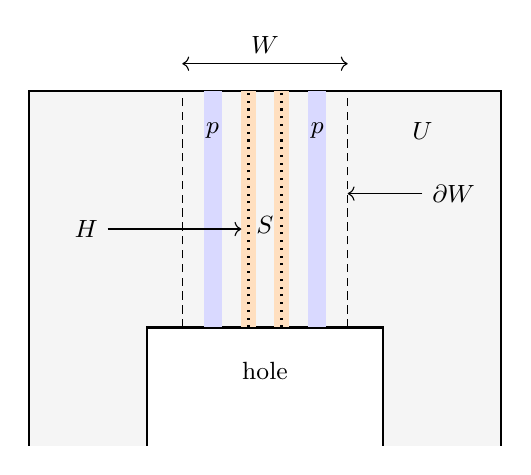
\begin{tikzpicture}[x=1cm,y=1cm,font=\small]
  \fill[gray!8] (-3,-1.5) rectangle (3,3);
  \fill[white] (-1.5,-1.5) rectangle (1.5,0);
  \draw[thick] (-3,-1.5)--(-3,3)--(3,3)--(3,-1.5);
  \draw[thick] (-1.5,-1.5)--(-1.5,0)--(1.5,0)--(1.5,-1.5);
  \fill[blue!15] (-.78,0) rectangle (-.55,3);
  \fill[blue!15] (.55,0) rectangle (.78,3);
  \fill[orange!25] (-.3,0) rectangle (-.12,3);
  \fill[orange!25] (.12,0) rectangle (.3,3);
  \draw[densely dashed] (-1.05,0)--(-1.05,3);
  \draw[densely dashed] (1.05,0)--(1.05,3);
  \draw[dotted,thick] (-.21,0)--(-.21,3);
  \draw[dotted,thick] (.21,0)--(.21,3);
  \node at (0,-.55) {hole};
  \node at (2,2.5) {\(U\)};
  \node at (0,1.3) {\(S\)};
  \node at (-.665,2.5) {\(p\)};
  \node at (.665,2.5) {\(p\)};
  \draw[->] (-2,1.25)--(-.3,1.25);
  \node[anchor=east] at (-2,1.25) {\(H\)};
  \draw[->] (2,1.7)--(1.05,1.7);
  \node[anchor=west] at (2,1.7) {\(\partial W\)};
  \draw[<->] (-1.05,3.35)--(1.05,3.35);
  \node[above] at (0,3.35) {\(W\)};
 \end{tikzpicture}
 \caption{A straight part of a strip \(S\) joining a hole to the
 outer free wall. Dotted lines indicate the interfaces cut to isolate
 \(S\). The pin region \(H\), shown along both interfaces, contains
 every endpoint of every lattice edge crossing either interface.
 The two
 guard bands \(p\) separate them from the artificial boundary of the
 wider patch \(W\). All bands have positive widths and positive
 intervening gaps. Parallel collars give the same separation at
 rectilinear turns. The bottom ends of the outer boundary and hole
 are omitted from the schematic.}
 \label{sectors:slit-figure}
\end{figure}


For prescribed absolute primary data \(u\) on \(p\), let
\[
 K^s(u)=\frac{Z_{\rm open}^s(u)}{Z_{\rm cut}^s(u)},
 \qquad d_0=K^0(0).
\]
Conditioning on the full guard separates the restored edges from
everything beyond \(W\), since no observation cell crosses a guard
division. Therefore \(K^s(u)\) is unchanged if we cut the edges
across \(\partial W\) and compute it using \(W\) alone.
The prescribed-data comparison of
Lemma~\ref{heights:cut-comparison} gives
\[
 \frac{Z_{\rm open}^s(u)}{Z_{\rm open}^0(0)}
 \le
 \frac{Z_{\rm cut}^s(u)}{Z_{\rm cut}^0(0)},
 \qquad\hbox{hence}\qquad 0<K^s(u)\le d_0.
\]

\emph{The loss inside the patch.}
Choose a union of positive-area boxes \(H\) containing all endpoints
of restored edges and positively separated from \(p\), in the cut
patch. Under its centered confined law,
\[
 1\ge \E_{{\rm cut}\,W,0}\frac{K^0(u)}{d_0}
 \ge e^{-D_{n,d}(H,p)}.
\]
To verify the lower bound, compare the restored partition sums with
guard data \(u\) and \(0\), then add the pin \(h_H=0\).
Precision comparison decreases their ratio. With \(H\) pinned,
restoration is a fixed scalar because all restored-edge endpoints
are fixed. Dividing by the corresponding cut-patch data ratio gives
the pointwise lower comparator
\[
 \frac{K^0(u)}{d_0}
 \ge
 \frac{\Pbb_{{\rm cut}\,W,0}(h_H=0\mid h_p=u)}
      {\Pbb_{{\rm cut}\,W,0}(h_H=0\mid h_p=0)}.
\]
Averaging and using Bayes' rule gives the displayed estimate.
Lemma~\ref{sectors:localization} shows that its lower bound tends
to one, in the order \(n\to\infty\), then \(d\downarrow0\).

Both versions of \(W\) have lifts, and the cuts remove only
zero-area interfaces. Lemma~\ref{sectors:single-lift} therefore
gives the same limit for their shifted-to-centered ratios.
It follows that
\begin{equation}
 \sum_u\frac{Z_{{\rm cut}\,W}^s(u)}{Z_{{\rm cut}\,W}^0}
           \left(1-\frac{K^s(u)}{d_0}\right)\longrightarrow0
 \quad(n\to\infty,\ \text{then }d\downarrow0).
 \tag{6}\label{eq:source-6}
\end{equation}
The arrow means that the iterated limsup is zero.
For clarity, the sum in Equation~\eqref{eq:source-6} is exactly
\[
 F_{{\rm cut}\,W}^s-
 F_{{\rm open}\,W}^s\,
       \E_{{\rm cut}\,W,0}\frac{K^0}{d_0}.
\]
This identity proves the assertion without any approximation of
conditional laws at individual microscopic values \(u\).

\emph{Passing from the patch to the whole domain.}
Let \(G\) be the current topology with the narrow strip cut, and
let \(G'\) be obtained by further cutting the edges across the
artificial boundary of \(W\). At prescribed guard data, precision
comparison gives
\[
 \frac{Z_G^s(u)}{Z_G^0(0_p)}
 \le \frac{Z_{G'}^s(u)}{Z_{G'}^0(0_p)}.
\]
Here \(0_p\) denotes prescribed zero guard data; a denominator without
a data argument sums over those data. Thus
\begin{equation}
 \frac{Z_G^s(u)}{Z_G^0}
 \le
 \frac{\Pbb_{G,0}(h_p=0)}{\Pbb_{G',0}(h_p=0)}
 \frac{Z_{G'}^s(u)}{Z_{G'}^0}.
 \label{sectors:global-data-bound}
\end{equation}
This change of normalization has a controlled cost.
Let \(R(u)\) be the centered restoration factor from \(G'\) to \(G\)
at guard data \(u\). Directly summing partition functions gives
\[
 \frac{\Pbb_{G,0}(h_p=0)}{\Pbb_{G',0}(h_p=0)}
 =\frac{R(0)}{\E_{G',0}R}.
\]
Choose a union of boxes \(H'\) containing the endpoints of all
edges across the artificial boundary of \(W\), separated from \(p\).
The preceding centered restoration comparison, now with \(H'\),
implies
\[
 \frac{\E_{G',0}R}{R(0)}
 \ge e^{-D_{n,d}^{G'}(H',p)}.
\]
Lemma~\ref{sectors:localization} makes this interaction tend to zero.
All observation cells remain within their components after the cut,
and control their constants, so its hypotheses hold for \(G'\).

Multiply Equation~\eqref{sectors:global-data-bound} by the
nonnegative quantity \(1-K^s(u)/d_0\) and sum.
On \(G'\), the part outside \(W\) factors off as a
shifted-to-centered confined ratio, at most one by
Lemma~\ref{heights:finite-comparisons}.
The resulting global loss is therefore at most
\(e^{D_{n,d}^{G'}(H',p)}\) times the patch loss in
Equation~\eqref{eq:source-6}; it tends to zero.
The same conclusion applies to the centered loss.

To finish, define these two losses on the current cut graph by
\[
 L_s=\sum_u\frac{Z_{\rm cut}^s(u)}{Z_{\rm cut}^0}
                 \left(1-\frac{K^s(u)}{d_0}\right),
 \qquad
 L_0=\E_{{\rm cut},0}\left(1-\frac{K^0}{d_0}\right).
\]
Summing the restored numerator and denominator gives the exact identity
\begin{equation}
 F_{\rm open}^s=\frac{F_{\rm cut}^s-L_s}{1-L_0}.
 \label{sectors:restoration-identity}
\end{equation}
Since \(L_s,L_0\) tend to zero in the prescribed order and
\(F_{\rm cut}^s\le1\), a strip deletion changes the confined ratio
by a quantity tending to zero. There are only finitely many strips.
After all deletions, Lemma~\ref{sectors:single-lift} identifies the
product ratio with the right side of Equation~\eqref{eq:source-5}.
The energies add over the pieces to \(\int_U|dv|^2\).
Restoring the strips proves the proposition. The raw factors \(d_0\)
cancel in Equation~\eqref{sectors:restoration-identity}; no bound on
their size is needed.
\end{proof}

\begin{proof}[Completion of Theorem~\ref{sectors:positive-radius}]
For every smooth \(g\) near \(\overline U\), combine
Equation~\eqref{sectors:confinement-lower} with
Proposition~\ref{sectors:weighted} to obtain
\[
 \liminf_{n\to\infty}F_{U,n}^s
 \ge \exp\left\{-\frac1{2a}\int_U|dv_0+dg|^2\right\}.
\]
Restrictions of smooth functions from a neighborhood are dense in
\(H^1(U)\), since \(U\) is Lipschitz. Let their energies approach
\(\mathcal M(U)\). This proves the lower bound in
Equation~\eqref{eq:source-3}, and the earlier upper bound proves the
limit. Every use of a height or pin theorem was at fixed geometry
and fixed \(d\); all subsequent limits were taken afterwards.
\end{proof}

\section{Flat pins across a long annulus}\label{sec:annuli}

The comparison in Theorem~\ref{sectors:positive-radius} concerns holes of
fixed positive radius. To connect such a hole to a microscopic source,
we need a pin-probability estimate on a long annulus: making the heights
equal on a middle band changes the probability that the heights are
equal at a distant end by a factor tending to one in the mesh limit
as the logarithmic annular length grows. Each of these events leaves
its common height free. We derive this estimate from
the absolute-pin input in Theorem~\ref{heights:pin-input}.

\subsection{Polygonal annuli and their bands}

Fix a small \(\varepsilon>0\), and choose a closed rectilinear polygon
\(P\), homeomorphic to a closed disk, with dyadic vertices and
\[
 B(0,1-\varepsilon)\subset P\subset B(0,1+\varepsilon).
\]
One may use a sufficiently fine staircase approximation to the circle,
chosen symmetrically in the four quadrants. All side lengths and
passages in the resulting fixed geometry are nondegenerate. Write
\(Q_r=(-r,r)^2\). Choose \(\lambda\) to be a sufficiently large power
of \(4\), and put
\[
 \begin{gathered}
 A_\lambda=\lambda P\setminus P^\circ,\qquad
 p=\overline{Q_{2\sqrt\lambda}}\setminus Q_{\sqrt\lambda},\\
 H_{\mathrm{in}}=A_\lambda\cap\overline{Q_4},\qquad
 H_{\mathrm{out}}=A_\lambda\setminus Q_{\lambda/4}.
 \end{gathered}
\]
Sobolev spaces on \(A_\lambda\) refer to its interior.
The guard \(p\) is a full square band separating the two ends.
Each end region contains all vertices next to its annular wall after
fine discretization. The guard and either end are positively separated.
They are finite unions of positive-area boxes in the polygonal
geometry of Section~\ref{sec:heights}. Discretizations use the coherent
array divisions specified there. In particular, a boundary division
never identifies pieces merely at a point.
Figure~\ref{annuli:figure} displays these regions.

\begin{figure}[tb]
 \centering
 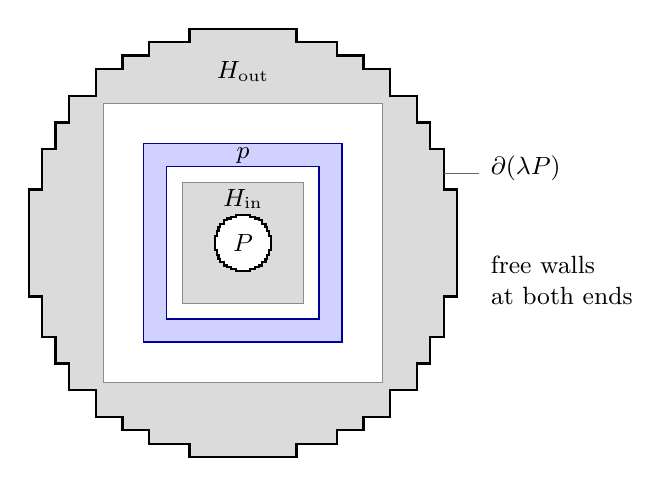
\begin{tikzpicture}[scale=.68, every node/.style={font=\small}]
 \def\wall{(4,0)--(4,1)--(3.75,1)--(3.75,1.75)
 --(3.5,1.75)--(3.5,2.25)--(3.25,2.25)--(3.25,2.75)
 --(2.75,2.75)--(2.75,3.25)--(2.25,3.25)--(2.25,3.5)
 --(1.75,3.5)--(1.75,3.75)--(1,3.75)--(1,4)
 --(-1,4)--(-1,3.75)--(-1.75,3.75)--(-1.75,3.5)
 --(-2.25,3.5)--(-2.25,3.25)--(-2.75,3.25)--(-2.75,2.75)
 --(-3.25,2.75)--(-3.25,2.25)--(-3.5,2.25)--(-3.5,1.75)
 --(-3.75,1.75)--(-3.75,1)--(-4,1)--(-4,-1)
 --(-3.75,-1)--(-3.75,-1.75)--(-3.5,-1.75)--(-3.5,-2.25)
 --(-3.25,-2.25)--(-3.25,-2.75)--(-2.75,-2.75)--(-2.75,-3.25)
 --(-2.25,-3.25)--(-2.25,-3.5)--(-1.75,-3.5)--(-1.75,-3.75)
 --(-1,-3.75)--(-1,-4)--(1,-4)--(1,-3.75)
 --(1.75,-3.75)--(1.75,-3.5)--(2.25,-3.5)--(2.25,-3.25)
 --(2.75,-3.25)--(2.75,-2.75)--(3.25,-2.75)--(3.25,-2.25)
 --(3.5,-2.25)--(3.5,-1.75)--(3.75,-1.75)--(3.75,-1)
 --(4,-1)--cycle}
 \fill[black!14] \wall;
 \fill[white] (-2.6,-2.6) rectangle (2.6,2.6);
 \fill[blue!18] (-1.85,-1.85) rectangle (1.85,1.85);
 \fill[white] (-1.42,-1.42) rectangle (1.42,1.42);
 \fill[black!14] (-1.125,-1.125) rectangle (1.125,1.125);
 \draw[black!45] (-2.6,-2.6) rectangle (2.6,2.6);
 \draw[blue!60!black] (-1.85,-1.85) rectangle (1.85,1.85);
 \draw[blue!60!black] (-1.42,-1.42) rectangle (1.42,1.42);
 \draw[black!45] (-1.125,-1.125) rectangle (1.125,1.125);
 \draw[thick] \wall;
 \begin{scope}[scale=.13]
  \fill[white] \wall;
  \draw[thick] \wall;
 \end{scope}
 \node at (0,0) {\(P\)};
 \node at (0,.82) {\(H_{\mathrm{in}}\)};
 \node at (0,1.64) {\(p\)};
 \node at (0,3.2) {\(H_{\mathrm{out}}\)};
 \node[anchor=west] at (4.45,1.4) {\(\partial(\lambda P)\)};
 \draw[black!60] (4.4,1.3)--(3.75,1.3);
 \node[anchor=west,align=left] at (4.45,-.7)
    {free walls\\at both ends};
\end{tikzpicture}

 \caption{A polygonal annulus with its full square guard \(p\) and the
 two possible end regions. The inner and outer walls are rectilinear
 approximations to circles; the square boundaries belong to the
 bands, not to the annular walls. Radial distances are compressed:
 the actual walls are \(P\) and \(\lambda P\), the guard is at scale
 \(\sqrt\lambda\), and either end is separated from it by a round
 annulus of logarithmic length
 \(\frac12\log\lambda-O(1)\). The two end regions are displayed
 together, but the pin estimate is applied to one end at a time.}
 \label{annuli:figure}
\end{figure}

Consider the centered, free height law \(\mu\) on this annulus, with
one common translation quotiented out. For a nonempty vertex set \(Q\),
write
\[
 [Q]=\{h_x=h_y\text{ for every }x,y\in Q\}.
\]
Thus \([Q]\) pins all differences within \(Q\), without pinning its
common height. For \(H=H_{\mathrm{in}}\) or \(H_{\mathrm{out}}\), set
\[
 \overline D(H,p)
   =\log\frac{\mu([H]\mid[p])}{\mu([H])}.
\]

\begin{proposition}[Separated flat pins]\label{annuli:flat-interaction}
Fix \(P\) as above. For either choice of \(H\), the interaction
\(\overline D(H,p)\) is nonnegative and
\begin{equation}
 \limsup_{\mathrm{mesh}\to0}\overline D(H,p)
 \quad\text{can be made arbitrarily small by taking \(\lambda\) large.}
 \tag{7}\label{eq:source-7}
\end{equation}
The mesh limit is taken at each fixed polygonal geometry.
\end{proposition}

The proof of Proposition~\ref{annuli:flat-interaction} first estimates
the continuum interaction with one confining
box average. It then weakens that confinement and passes from absolute
pins to flat pins. The constant mode is retained throughout.

\subsection{The continuum estimate with confinement}

Choose a dyadic box inside \(p\) whose side lengths are fixed positive
multiples of \(\sqrt\lambda\), and let \(B_0\) be its probability
average. Sum all common height translations and add the penalty
\(\gamma(B_0h)^2/2\), where \(\gamma>0\). Let \(D_\gamma(H,p)\)
be the interaction of the absolute events \(h_H=0\) and \(h_p=0\)
under this confined law.

Start with \(\gamma=1\). By Theorem~\ref{heights:pin-input},
\(D_1\) converges to the Gaussian
interaction for
\[
 \mathcal T(u)=a^{-1}\int_{A_\lambda}|\nabla u|^2+(B_0u)^2.
\]
Write \(\|u\|_{\mathcal T}^2=\mathcal T(u)\).
As in Equation~\eqref{eq:source-1}, let
\[
 V_Q=\{u\in H^1(A_\lambda):u=0\text{ on }Q\}^{\perp_{\mathcal T}},
 \qquad C=\Pi_H|_{V_p}.
\]
We claim that \(\|C\|_{\mathrm{HS}}\to0\) as \(\lambda\to\infty\).

Between \(p\) and \(H\) there is a full round annulus which is a
conformal cylinder
\begin{equation}\label{annuli:cylinder}
 [0,T]\times\bigl(\R/(2\pi\Z)\bigr),\qquad
 T=\tfrac12\log\lambda-O(1).
\end{equation}
The end \(s=0\) faces \(p\). For the inner end, for example, one may
take radii \(8\) and \(\sqrt\lambda/2\), with the logarithmic coordinate
reversed. For the outer end one may take radii \(4\sqrt\lambda\) and
\(\lambda/8\). Enlarging the lower bound on \(\lambda\) makes both
choices available, with fixed clearances from the bands.

For \(f\in V_p\), the trace at \(s=0\) satisfies
\begin{equation}\label{annuli:trace}
 \|f|_{s=0}\|_{H^{1/2}(\mathbb S^1)}
       \le C_0\|f\|_{\mathcal T},
\end{equation}
with \(C_0\) independent of large \(\lambda\). Indeed, after scaling
lengths by \(\sqrt\lambda\), this circle, the guard, and the observation
box lie in a fixed connected annular region. Poincare's inequality
with the box mean controls the \(H^1\) norm there, including constants;
the trace theorem then gives Equation~\eqref{annuli:trace}.
On the side of this circle containing \(H\), the function \(f\)
minimizes the gradient energy with its given trace and free walls.
There is no observation term on that side.

Let \(A\) map a trace at \(s=0\) to the restriction to \(H\) of this
energy minimizer, with the target norm equal to the least
\(\mathcal T\)-norm of an extension of that restriction to the whole
annulus. This target is naturally identified with \(V_H\).
We estimate \(A\) on a normalized Fourier basis of \(H^{1/2}(\mathbb S^1)\).
For the constant trace, the minimizer on the \(H\)-side is constant.
An extension of its \(H\)-data can be chosen constant beyond \(s=T\),
linear across the cylinder, and zero before \(s=0\). It vanishes on
the observation box and has energy \(O(T^{-1})\). Thus the norm of
the image of the constant mode is \(O(T^{-1/2})\).

For a sine or cosine mode of frequency \(j\ge1\), normalization in
\(H^{1/2}\) makes its amplitude \(O((1+j)^{-1/2})\).
The Neumann minimum at \(s=T\), on the cylinder alone, is a lower
bound for the actual minimum. The Dirichlet-zero minimum at \(s=T\),
extended by zero beyond that circle, is an admissible upper trial.
The solutions of \(u''=j^2u\) give, respectively, the factors
\(\tanh(jT)\) and \(\coth(jT)\) in their energies. Their difference
is therefore \(O(e^{-2jT})\). Orthogonality of the actual minimizer
to zero-trace variations shows that the difference between it and
the upper trial has gradient norm \(O(e^{-jT})\). This difference
has zero trace at \(s=0\), so it extends by zero toward \(p\), pays no
observation penalty, and has, up to sign, the required restriction
on \(H\). Consequently
\[
 \|A\|_{\mathrm{HS}}^2
       \le \frac{C_1}{T}+C_1\sum_{j\ge1}e^{-2jT}
       \longrightarrow0.
\]
All extensions are in \(H^1\): across each interior circle their
traces agree. Composing \(A\) with the uniformly bounded trace map
in Equation~\eqref{annuli:trace} proves the claim for \(C\).
The determinant in Equation~\eqref{eq:source-1} now tends to one,
since \(\|C\|\le\|C\|_{\mathrm{HS}}\to0\). We have proved
\begin{equation}\label{annuli:unit-confinement}
 \lim_{\lambda\to\infty}\lim_{\mathrm{mesh}\to0}D_1(H,p)=0.
\end{equation}

\subsection{From absolute pins to flat pins}

We next establish Equation~\eqref{annuli:unit-confinement} with any
fixed \(\gamma>0\) in place of \(1\). Consider the four partition
functions defining the absolute-pin interaction. When \(p\) is
pinned, \(B_0h=0\), so changing \(\gamma\) has no effect. With neither
region pinned, the ratio of partition functions at precisions
\(\gamma\) and \(1\) tends to \(\gamma^{-1/2}\). This follows from
Theorem~\ref{heights:mixed-input}: the fractional mean becomes uniform and
independent of the mean-free field, and the translation sums of the
Gaussian penalties are bounded periodic functions.

With \(H\) alone pinned, let \(x=x(\lambda)\) be the variance of \(B_0\)
in the massless continuum Gaussian law with that pin. Applying the
hard-pin height limit in Theorem~\ref{heights:mixed-input} to the two bounded weights
\(\exp(-\gamma(B_0h)^2/2)\) and \(\exp(-(B_0h)^2/2)\) gives the ratio
\[
 \left(\frac{1+x}{1+\gamma x}\right)^{1/2}.
\]
Moreover \(x\to\infty\). To see this from the variational formula for
the variance, take a function equal to one on the \(p\)-side, zero
on the \(H\)-side, and linear across the cylinder
in Equation~\eqref{annuli:cylinder}. Its box average is one and
its gradient energy is \(O(T^{-1})\), so \(x\ge cT\).
Combining the four partition functions yields, at fixed geometry,
\begin{equation}\label{annuli:change-confinement}
 D_\gamma-D_1\longrightarrow
       \frac12\log\frac{1+\gamma x}{\gamma(1+x)}.
\end{equation}
The right side tends to zero as \(\lambda\to\infty\). The absolute-pin
interaction thus tends to zero for every fixed positive \(\gamma\).

It remains to compare these absolute pins with the desired flat
events. In a centered confined law, the logarithmic interaction of
two centered quadratic penalties increases when either precision
increases. In fact, if the first precision changes by \(tQ\),
differentiating the four log partition functions gives
\[
 \frac12\Tr Q\bigl(\Cov_{\text{first penalty}}
                    -\Cov_{\text{both penalties}}\bigr)\ge0
\]
by centered covariance comparison. Taking equality limits proves
the same assertion for nested centered constraints. Absolute zero
pins are obtained from flat pins by also pinning one reference
height in each set after the within-set constraints are imposed.
Hence the interaction of \([H]\) and \([p]\)
in the confined law is between zero and \(D_\gamma(H,p)\).

Finally, project the confined law onto common-translation orbits.
If \(t=B_0h\) in any representative, the orbit receives the factor
\[
 w_\gamma(t)=\sum_{k\in\Z}
       \exp\{-\tfrac{\gamma}{2}(t+2\pi k)^2\}.
\]
Poisson summation gives the uniform estimate
\[
 \sup_t\left|\sqrt{2\pi\gamma}\,w_\gamma(t)-1\right|
 \le 2\sum_{j\ge1}e^{-j^2/(2\gamma)}
       =:\delta_\gamma\longrightarrow0
       \qquad(\gamma\downarrow0).
\]
For \(\gamma\) sufficiently small that \(\delta_\gamma<1\), the
normalized projected density relative to the free
orbit law is between
\((1-\delta_\gamma)/(1+\delta_\gamma)\) and its reciprocal.
This multiplicative estimate applies to the individual pin events
and their intersection, however small their probabilities. Their
log interactions differ by \(O(\delta_\gamma)\), uniformly in the
mesh and the annulus.

Given a tolerance, first choose \(\gamma>0\) so that this error is
small. Then choose \(\lambda\) large so that the limiting absolute-pin
interaction is small, and finally take the mesh limit at that
fixed geometry. This proves Equation~\eqref{eq:source-7}.
Nonnegativity in the free law follows either from centered
precision comparison directly or by sending \(\gamma\) to zero
at each fixed finite graph.
\qed

\section{Gluing kernels and stability from a fixed core}\label{sec:kernels}

We now return to the bare height weights, with no confining penalty.
The flat-pin estimate gives an average bound for restoring an interface
between annuli. A uniform upper bound for the same kernel will make
that estimate stable through any number of annuli.

\subsection{Guard data and interface kernels}

Use the polygon \(P\), the guard, and the end regions of
Section~\ref{sec:annuli}. In lattice units, an annular block has walls
\(RP\) and \(\lambda RP\). We take \(R\) large enough and dyadically
aligned so that all divisions lie between rows of dual vertices.
Every block is connected. The bonds between adjacent blocks are
precisely the bonds to be restored.

Choose one guard vertex in each annulus. Its \emph{guard datum}
\(u\) is the list of all height differences from that vertex to the
other guard vertices, in the chosen connection gauge. Every
compatible datum has positive probability. Denote its law in block
\(i\), in sector \(s\), by \(m_i^s(du)\). Fixing the representative
whose chosen height is zero turns \(u\) into full prescribed height
data on the guard. The configurations on the two sides are then
conditionally independent, since the guard is a full separating
band and the energy is a sum of nearest-neighbor terms.

For two adjacent annuli, with data \(u_i,u_{i+1}\), define
\[
 T_i^s(u_i,u_{i+1})
   =\frac{Z_{\mathrm{restored}}^s(u_i,u_{i+1})}
           {Z_{\mathrm{cut}}^s(u_i,u_{i+1})}.
\]
The numerator is summed modulo one common translation; the
denominator is a product of sums modulo one translation in each
block. Thus the numerator sums the relative integer translation
of the two blocks.

We use the same definition in two other cases. A \emph{core} is
a connected block filling the inner hole of the first annulus;
it may contain a magnetic source and carries no prescribed guard.
Its interface kernel is a function \(T_0^s(u_1)\). At the other
end, several disjoint last annuli may be attached to one connected
exterior, with no direct bonds between these annuli. The exterior
carries no prescribed data. Its one joint kernel is a function of
the incident annular data. In every case let
\[
 d_i=T_i^0(0),
\]
where \(0\) means zero guard differences in the centered sector.
No size estimate for this positive scalar is required.

\begin{lemma}[Upper bound and centered average]\label{kernels:bounds}
For each of the kernels just defined, every sector and every
compatible guard datum satisfy
\begin{equation}
                  0<T_i^s/d_i\le1. \tag{8}\label{eq:source-8}
\end{equation}
For an interface between two annuli, choose the end region \(H\)
on each side containing its seam endpoints. For the joint exterior
kernel choose the outer end region in each incident annulus. Then
\begin{equation}
 1\ge \int (T_i^0/d_i)
                 \prod_{\text{incident annuli }\ell}dm_\ell^0
 \ge \prod_{\text{incident annuli }\ell}
                    e^{-\overline D_\ell(H,p)} .
 \tag{9}\label{eq:source-9}
\end{equation}
\end{lemma}

\begin{proof}
Lemma~\ref{heights:cut-comparison} gives the prescribed-data comparison
\[
 \frac{Z_{\mathrm{restored}}^s(u)}
      {Z_{\mathrm{restored}}^0(0)}
 \le
 \frac{Z_{\mathrm{cut}}^s(u)}{Z_{\mathrm{cut}}^0(0)}.
\]
Rearranging proves Equation~\eqref{eq:source-8}. The comparison
applies to relative guard data: they are affine constraints on
height differences. If auxiliary confinement is used to perform
the comparison, its divergent translation scalar cancels within
each displayed ratio before confinement is removed. The two graphs
need not have the same number of free components.

For the lower bound, work in the centered sector and impose \([H]\)
in every indicated annulus. Adding these centered constraints to
the restored data-versus-zero ratio decreases that ratio. Once they
hold, choose the representative in each annulus to be zero on
its flat end. The restoration factor is then independent of the
guard data: its remaining variables are the relative integer
translations and, in the exterior case, the unprescribed exterior
heights. Let \(\Pbb_{\ell,0}\) denote the free centered law in
annulus \(\ell\). The comparison, after division by the cut
data-versus-zero ratio, gives
\[
 \frac{T_i^0(u)}{d_i}
 \ge
 \prod_{\text{incident annuli }\ell}
 \frac{\Pbb_{\ell,0}([H]\mid u_\ell)}
      {\Pbb_{\ell,0}([H]\mid[p])}.
\]
All seam endpoints lie in the chosen end regions; hence no other
annular heights enter the restoration factor with these events
imposed. Averaging over the independent cut-block laws yields
Equation~\eqref{eq:source-9}.
\end{proof}

\begin{lemma}[Exact multiplication]\label{kernels:multiplication}
Let a core be surrounded by \(N\) annular blocks, with no other
adjacencies between the blocks. Their restored partition function is
\begin{equation}\label{kernels:product}
 Z_{\mathrm{full}}^s
 = Z_{\mathrm{core}}^s\prod_{i=1}^N Z_i^s
   \int T_0^s(u_1)
         \prod_{i=1}^{N-1}T_i^s(u_i,u_{i+1})
         \prod_{i=1}^N dm_i^s(u_i).
\end{equation}
For several disjoint nests attached to a common connected exterior,
the corresponding formula includes its cut partition function and
the one joint exterior kernel.
\end{lemma}

\begin{proof}
Begin with one representative of the heights in each cut block.
On the tree whose vertices are these blocks and whose edges are
their interfaces, integer block constants modulo one common
constant are in bijection with the integer differences along the
tree edges. The bijection has no multiplicity factor: fix the
root constant, then recover each other constant along its unique
path from the root. The relative translations can therefore be
summed independently at the interfaces.

Condition next on every guard datum. Within each annulus, its inner
and outer configurations are conditionally independent. The two
incident interface factors may consequently be integrated separately,
giving the kernels in Equation~\eqref{kernels:product}. For several
nests, put the exterior at the root of the block tree. Its different
boundary portions need not be independent, so their integrations
remain together in the single exterior kernel. This is exactly the
formula asserted.
\end{proof}

\subsection{Small average losses in unit magnetic sectors}

Call an annulus-annulus interface \emph{regular} when the connection
is flat on their restored union and has the same period \(2\pi\),
\(-2\pi\), or zero in both annuli. In particular, restoring that
interface introduces no magnetic source.

\begin{proposition}[Average loss]\label{kernels:average-loss}
For a regular interface,
\begin{equation}
 \int(T_i^s/d_i)\prod_\ell dm_\ell^s
 =
 \left(\int(T_i^0/d_i)\prod_\ell dm_\ell^0\right)
       \frac{F_{\mathrm{restored}}^s}{F_{\mathrm{cut}}^s}.
 \tag{10}\label{eq:source-10}
\end{equation}
Given any \(\xi>0\), first choose \(\varepsilon\) sufficiently small
and fix a polygon \(P\) satisfying its disk inclusions. Then choose
\(\lambda\) sufficiently large. There is a fixed aligned
threshold \(R_0\) such that every regular interface with smaller
inner scale at least \(R_0\) satisfies
\begin{equation}
             \int(1-T_i^s/d_i)\prod_\ell dm_\ell^s\le\xi
 \tag{11}\label{eq:source-11}
\end{equation}
in each of the two unit-period sectors and in the centered sector.
The individual flat-pin interactions in
Equation~\eqref{eq:source-9} can also be made arbitrarily small
with these choices.
\end{proposition}

\begin{proof}
The integral of \(T_i^s\) under the independent cut-block laws is
\(Z_{\mathrm{restored}}^s/Z_{\mathrm{cut}}^s\). Dividing this
identity by its centered counterpart proves
Equation~\eqref{eq:source-10}. The same identity is valid for a
joint exterior kernel, without a claim yet about its average loss.

For a circular annulus of radii \(1\) and \(\lambda\), the minimum
energy with unit period \(2\pi\) is \(2\pi\log\lambda\).
The angular function attains it, and integration on concentric
circles proves the matching lower bound. Restriction of admissible
forms, together with
\(B(0,1-\varepsilon)\subset P\subset B(0,1+\varepsilon)\), gives
\[
 \mathcal M(\lambda P\setminus P^\circ)
       =2\pi\log\lambda+O(\varepsilon),
\]
where the constant is independent of large \(\lambda\). For example,
the circular annulus with radii \(1+\varepsilon\) and
\(\lambda(1-\varepsilon)\) is contained in the polygonal one,
which in turn is contained in the circular annulus with radii
\(1-\varepsilon\) and \(\lambda(1+\varepsilon)\).
The same bounds apply with \(\lambda^2\) to the union of two blocks.
It follows that
\[
 0\le
 \mathcal M(\lambda^2P\setminus P^\circ)
       -2\mathcal M(\lambda P\setminus P^\circ)
 \le C\varepsilon.
\]
The lower bound follows by restriction to the two cut annuli;
their energies agree by scale invariance in dimension two.
Theorem~\ref{sectors:positive-radius}, applied at this fixed geometry,
therefore makes the last factor in Equation~\eqref{eq:source-10}
converge to a number in \([e^{-C\varepsilon/(2a)},1]\).
Changing the unit period's sign does not change its energy.

Choose \(\varepsilon\) to make this error small, and then choose
\(\lambda\) so that Proposition~\ref{annuli:flat-interaction} makes
the two centered pin interactions small.
Equation~\eqref{eq:source-9} and
Equation~\eqref{eq:source-10} now give the desired small loss in
the mesh limit. With \(P\) and \(\lambda\) fixed, every regular
interface is a refinement of one fixed geometry. The convergence
theorems hold along every admissible mesh sequence, so there is
one threshold \(R_0\) beyond which the inequalities hold at every
aligned scale. There are only three sectors to consider.
This proves Equation~\eqref{eq:source-11}.
\end{proof}

\subsection{A positive-kernel stability lemma}

The preceding estimate controls the average loss under independent
guard laws. Actual guard data in a nest have been influenced by
all the inner blocks. The following lemma bounds that change of law
without accumulating a fixed error at every interface.

\begin{lemma}[Stability from a positive initial weight]
\label{kernels:stability}
Let \((X_i,m_i)\), \(i\ge1\), be probability spaces, and let
\(t_i:X_i\times X_{i+1}\to(0,1]\) be measurable kernels with
\[
 \int(1-t_i)\,d(m_i\otimes m_{i+1})\le\xi,\qquad
                         0<\xi<1/64.
\]
Fix a measurable \(g:X_1\to(0,1]\), positive \(m_1\)-almost
everywhere. For each \(N\), give \(X_1\times\cdots\times X_N\)
density proportional to
\[
                    g(u_1)\prod_{i=1}^{N-1}t_i(u_i,u_{i+1})
\]
with respect to \(\prod_i m_i\). For all sufficiently large \(N\),
its last-coordinate marginal has density at most \(2\) with respect
to \(m_N\). No positive essential lower bound on \(g\) is required.
\end{lemma}

\begin{proof}
Define
\[
 L_i f(v)=\int t_i(u,v)f(u)\,dm_i(u).
\]
First propagate the constant density:
\[
 q_1=1,\qquad
 \beta_i=\int L_iq_i\,dm_{i+1},\qquad
 q_{i+1}=\beta_i^{-1}L_iq_i.
\]
Inductively \(q_i\le2\), because
\[
 \beta_i
  =1-\int(1-t_i)q_i\,d(m_i\otimes m_{i+1})
  \ge1-2\xi,\qquad
 q_{i+1}\le M:=(1-2\xi)^{-1}<2.
\]
The same argument, with the kernels reversed, bounds by \(2\) any
normalized density obtained by propagating \(1\) backwards through
a finite number of them.

Propagate \(g\) using these same scalars, rather than renormalizing
it at each step:
\[
 f_1=g,\qquad f_{i+1}=\beta_i^{-1}L_if_i,\qquad
 c_i=\int f_i\,dm_i,\qquad E_i=f_i-c_iq_i.
\]
The scalar \(c_i\) is the ratio of the two integrals obtained by
starting with \(g\) and with \(1\). Equivalently, it is the
expectation of \(g\) under a normalized backwards density on
\(X_1\), which is at most \(2\). Choose \(\delta>0\) with
\(m_1(g<\delta)<1/4\). Every such density assigns at least half
its mass to \(\{g\ge\delta\}\), so
\begin{equation}\label{kernels:core-mass}
                         c_i\ge\delta/2
                    \quad\text{for every }i.
\end{equation}

For a mean-zero function \(E\), replace \(t_i\) in \(L_iE\) by
\(t_i-1\). Since \(0\le(1-t_i)^2\le1-t_i\), the resulting
operator has \(L^2(m_i)\)-to-\(L^2(m_{i+1})\) norm at most
\(\sqrt\xi\). The exact recurrence for the centered remainder is
\[
 E_{i+1}
 =\frac{L_iE_i-\bigl(\int L_iE_i\,dm_{i+1}\bigr)q_{i+1}}
        {\beta_i}.
\]
Using \(\|q_{i+1}\|_2\le2\), we obtain
\begin{equation}\label{kernels:contraction}
 \|E_{i+1}\|_2
 \le\frac{3\sqrt\xi}{1-2\xi}\|E_i\|_2.
\end{equation}
The factor is strictly smaller than one. Also \(t_i\le1\) gives
\(\|L_iE_i\|_\infty\le\|E_i\|_2\), and hence
\[
 \|E_{i+1}\|_\infty
       \le\frac{3}{1-2\xi}\|E_i\|_2.
\]
Thus the remainders tend to zero in the last displayed norm.
The last-coordinate density in the lemma is
\[
                    f_N/c_N=q_N+E_N/c_N.
\]
Equation~\eqref{kernels:core-mass} and the strict inequality
\(M<2\) show that it is eventually bounded by \(2\).
\end{proof}

\subsection{Application to a nest of annuli}

Fix the parameters in Proposition~\ref{kernels:average-loss} with
\(\xi<1/64\), and increase the aligned \(R_0\) if necessary. Set
\[
                 R_j=R_0\lambda^j,\qquad j\ge0.
\]
Let annulus \(i\) have walls \(R_{i-1}P\) and \(R_iP\), and fill
the inner hole by the fixed core in \(R_0P\). The core is a fixed
finite graph in lattice units. In a unit magnetic sector it
contains the source; all regular annuli carry its period.
Fix the core and the connection on the increasing family of blocks
once and for all, so restrictions agree as the depth \(N\) increases.
A fixed straight connection cut from the source gives such a choice.
Thus the first guard law and its core interface kernel do not vary
with \(N\).

\begin{corollary}[The last guard law]\label{kernels:last-guard}
For these fixed choices, the last-guard law in a nest of \(N\)
annuli has density at most \(2\) relative to \(m_N^s\) for all
sufficiently large \(N\), in the centered sector and in either
unit-period sector. The conclusion holds for identical lattice
translates of the nest with the same threshold in \(N\).
\end{corollary}

\begin{proof}
Put \(t_i=T_i^s/d_i\) for regular interfaces and
\(g=T_0^s/d_0\) for the core interface. Lemma~\ref{kernels:bounds}
gives \(0<g\le1\) and \(0<t_i\le1\).
Proposition~\ref{kernels:average-loss} gives the average-loss
hypothesis of Lemma~\ref{kernels:stability}.
Exact multiplication in Lemma~\ref{kernels:multiplication}
identifies its last marginal with the actual last-guard law.
The fixed initial weight \(g\) may be arbitrarily small on some
data; positivity is sufficient.

A lattice translation preserves all block laws and kernels.
Changing the source sign negates the connection and heights.
More generally, a connection with the same source restricts on
the nest to the chosen connection up to an integral gauge change,
which merely reindexes the guard data. Taking the maximum of the
finitely many thresholds for the centered and two unit sectors
proves the assertion.
\end{proof}

\section{Critical spin correlations}\label{sec:correlations}

The sector limit of Section~\ref{sec:sectors} and the gluing estimates
of Section~\ref{sec:kernels} now determine the spin correlations after
normalization by the center magnetization.  The microscopic part of
each unit source will be represented by an identical nest of annuli.
Its partition ratio need not have an asymptotic expansion: the same
ratio occurs in the center observable and cancels.

Throughout this section, \(k\geq1\) is fixed,
\(\sigma_i\in\{-1,1\}\), and
\[
 x_{i,n}\in D_n^\circ,\qquad x_{i,n}\longrightarrow z_i\in D,
 \qquad z_i\ne z_j\quad(i\ne j).
\]
Write the continuum Dirichlet Green kernel as
\[
 G_D(z,w)=\frac1{2\pi}\log\frac1{|z-w|}+R_D(z,w).
\]
The function \(R_D\) is smooth across the diagonal on compact subsets
of \(D\times D\).  Define
\[
 H_D(\mathbf z,\boldsymbol\sigma)
 =\sum_{i=1}^k R_D(z_i,z_i)
       +2\sum_{i<j}\sigma_i\sigma_jG_D(z_i,z_j).
\]
No assumption on \(\sum_i\sigma_i\) is imposed.

\subsection{The energy outside small holes}

\begin{lemma}[Exterior energy]\label{correlations:exterior-energy}
Remove the closed disks of radius \(\rho\) about the distinct points
\(z_1,\ldots,z_k\) from \(D\), where \(\rho>0\) is small enough that
these disks are disjoint and contained in \(D\).  For affine gradients
with periods \(2\pi\sigma_i\) about the holes, the minimum energy of
Equation~\eqref{eq:source-3} satisfies
\begin{equation}
 \mathcal M
 =2\pi k\log(1/\rho)
      +4\pi^2H_D(\mathbf z,\boldsymbol\sigma)+O(\rho).
 \tag{12}\label{eq:source-12}
\end{equation}
The error constant may depend on the separated interior configuration,
but is uniform for all sufficiently small \(\rho\).
\end{lemma}

\begin{proof}
Set \(U(y)=\sum_i\sigma_iG_D(y,z_i)\), and rotate
\(-2\pi\nabla U\) by a right angle, with the orientation chosen to give
the indicated periods.  Denote the resulting vector field by \(v\).
It is a smooth affine gradient on the punctured square, is divergence
free there, and is tangent to the outer boundary because \(U\) has
zero Dirichlet trace.  Thus \(v\) is an admissible trial field.

Near \(z_i\), write
\[
 U(y)=\frac{\sigma_i}{2\pi}\log\frac1{|y-z_i|}+u_i(y),
 \qquad
 u_i(z_i)=\sigma_iR_D(z_i,z_i)
                 +\sum_{j\ne i}\sigma_jG_D(z_i,z_j).
\]
The functions \(u_i\) are smooth and harmonic on fixed disjoint
neighborhoods of the sources.  On the boundary of a hole, the radial
singularity contributes no normal component to \(v\).  Its remaining
normal component is bounded uniformly in \(\rho\) and has integral
zero, since it is a tangential derivative of \(u_i\).

Let \(g\in H^1\) on the punctured square.  Integration by parts,
followed by subtraction of the mean of \(g\) on each inner circle,
gives
\[
 \left|\int v\cdot\nabla g\right|
 \leq C\rho\,\|\nabla g\|_2.
\]
Indeed, the \(L^2\) norm of \(v\cdot\nu\) on such a circle is
\(O(\rho^{1/2})\), whereas the trace and Poincar\'e inequalities on
the adjacent annulus of radii \(\rho\) and \(2\rho\) give
\[
 \|g-\text{its circle mean}\|_{L^2(\partial B(z_i,\rho))}
 \leq C\rho^{1/2}
        \|\nabla g\|_{L^2(B(z_i,2\rho)\setminus B(z_i,\rho))}.
\]
The collars are disjoint.  Minimizing
\(\|v+\nabla g\|_2^2\) therefore changes \(\|v\|_2^2\)
by at most \(O(\rho^2)\).

It remains to calculate
\(\|v\|_2^2=(2\pi)^2\int|\nabla U|^2\).
The outer-boundary contribution to Green's identity vanishes.
On the circle about \(z_i\), with \(\nu\) pointing into the hole,
the integral of \(U\partial_\nu U\) is
\[
 \frac1{2\pi}\log(1/\rho)+\sigma_i u_i(z_i)+O(\rho).
\]
The integral of the normal derivative of the regular harmonic part
is zero; in particular it produces no logarithmically enhanced
error.  Summing over the circles gives
Equation~\eqref{eq:source-12}.  These integrations may also be
performed with weak Dirichlet data on the outer square.  Alternatively,
reflection across its sides and corners, away from the sources,
justifies the boundary calculation directly.
\end{proof}

We shall apply this calculation to the rectilinear holes required by
the lattice decomposition.  Let \(P\) be the polygon chosen in
Section~\ref{sec:annuli}, so that
\[
 B(0,1-\varepsilon)\subset P\subset B(0,1+\varepsilon).
\]
Here and in the next lemma, radii are in the scaled coordinates of
\(D\), rather than in lattice units.

\begin{lemma}[Moving lattice holes]\label{correlations:exterior-lattice}
Suppose that \(\rho_n\to\rho>0\), where \(\rho\) is sufficiently
small.  Around \(x_{i,n}\), cut out the interiors in the array
division with hole shape \(\rho_nP\), using the rounding conventions
of Section~\ref{sec:sectors}.  Let \(F_{\rm ext}^s\) be the sector
ratio in the remaining dual graph, with periods
\(2\pi\sigma_i\) about these holes.  Then
\begin{equation}
 \limsup_n
 \left|
 \log F_{\rm ext}^s+
 \frac{2\pi k\log(1/\rho)+4\pi^2H_D(\mathbf z,\boldsymbol\sigma)}
      {2a}
 \right|
 \leq C(\varepsilon+\rho).
 \tag{13}\label{eq:source-13}
\end{equation}
The constant \(C\) depends on the separated limiting configuration
but not on sufficiently small \(\rho\) or \(\varepsilon\).
The same assertion holds after bounded-step mesh rounding.
\end{lemma}

\begin{proof}
Bracket the moving holes by fixed, positively separated rectilinear
holes with dyadic coordinates.  To obtain strict eventual inclusions,
start with circles of radii \((1-3\varepsilon)\rho\) and
\((1+3\varepsilon)\rho\) about the limiting points, and approximate
them and their centers by still smaller dyadic perturbations.
The perturbations can be chosen after fixing \(\rho\) and
\(\varepsilon\).  For all sufficiently large \(n\), the rounded
moving holes lie between these fixed approximations and contain
their respective sources.  The outer boundary remains the same square.

Use one connection before making any of these cuts.  Its restrictions
to the three exteriors have the same winding data.  The cut comparison
in Equation~\eqref{eq:source-2} therefore brackets their sector ratios.
Theorem~\ref{sectors:positive-radius} applies to each fixed polygonal
exterior.  Its continuum minimum energy is in turn bracketed by the
energies for the corresponding circular holes: restriction of an
admissible affine gradient preserves all the remaining periods.
Changing each radius by a factor \(1+O(\varepsilon)\) changes the
logarithmic term of Equation~\eqref{eq:source-12} by
\(O(\varepsilon)\).  That equation now proves the claim.

Every domain used in this argument has positive passages and
separated hole boundaries.  Coherent rounding consequently preserves
connectivity and the cycles defining the periods.  In particular the
argument uses only fixed-domain limits; it does not require uniform
convergence under arbitrary motion of the lattice marks.
\end{proof}

\subsection{Identical nests and their exterior attachment}

Fix the annular parameters \(\varepsilon,\lambda,R_0\) as in
Section~\ref{sec:kernels}, and write
\[
 R_j=R_0\lambda^j,\qquad
 N=N(n)=\max\{j:R_j\leq\eta n\},
\]
where \(\eta>0\) is small.  The \(R_j\) are now lattice radii.
Place identical translated nests, from their filled cores through
their \(N\)-th annuli, around all \(x_{i,n}\).
For sufficiently small \(\eta\), these nests have disjoint closures,
are contained in the spin square, and leave a connected exterior.
Use the same parameters and the same \(N\) for a single nest centered
at \(0\), which will represent the observable \(a_n\).
Since \(nx_{i,n}\in\Z^2\), the microscopic cores and all annuli are
exact lattice translates.  The restricted connections differ only
by integral gauge transformations; reversing a unit period also
leaves a bare nest ratio unchanged.

We may pass further along any subsequence so that
\[
 R_N/n\longrightarrow t\in[\eta/\lambda,\eta].
\]
For fixed \(\eta,\lambda\), this is a positive macroscopic radius.
The following estimate concerns only the joint kernel which attaches
the last annuli to the exterior.  Its notation is that of
Lemma~\ref{kernels:bounds}: \(d_{\rm ext}\) is the centered kernel
at zero relative guard data, and \(m_{N,i}^s\) is the cut law of
the last guard in the \(i\)-th annulus.

\begin{lemma}[Exterior attachment]\label{correlations:attachment}
For every sufficiently small \(\xi>0\), the parameters may be chosen
so that Equation~\eqref{eq:source-11} holds throughout the regular
annuli and
\begin{equation}
 \limsup_n\int
       \left(1-\frac{T_{\rm ext}^s}{d_{\rm ext}}\right)
                 \prod_{i=1}^k dm_{N,i}^s
 \leq\xi .
 \tag{14}\label{eq:source-14}
\end{equation}
This holds both for the shifted and centered calculations and for
the single center nest.  The parameters depend on the fixed
separated configuration and on \(\xi\), but not on \(n\).
The errors in Equation~\eqref{eq:source-13} at the radii in this
construction may simultaneously be made at most \(\xi\).
\end{lemma}

\begin{proof}
For the centered calculation, Equation~\eqref{eq:source-9} bounds
the attachment loss by the sum of the flat-pin interactions in
the incident last annuli.  These interactions can be made as small
as desired by the choices in Section~\ref{sec:annuli}.
The bound depends only on these annuli, not on the exterior.

For the shifted calculation use the exact identity
in Equation~\eqref{eq:source-10}, now for the last annuli together
with their common exterior.  Restoring them produces an exterior
whose smaller holes have radius parameter tending to \(t/\lambda\).
Before restoration, the factors are the \(k\) last-annulus sector
ratios and the exterior ratio with holes of radius parameter \(t\).
By Theorem~\ref{sectors:positive-radius}, each annular energy is
\(2\pi\log\lambda+O(\varepsilon)\).  By
Equation~\eqref{eq:source-13}, the restored and cut exterior energies
have the same term \(4\pi^2H_D(\mathbf z,\boldsymbol\sigma)\).
The difference between their radius terms is exactly
\(k\,2\pi\log\lambda\).  Consequently the logarithm of the
restored sector ratio divided by the product of the cut ratios
has absolute limiting error at most \(C(\varepsilon+\eta)\).
The circular energy brackets make this error uniform over
\(t\in[\eta/\lambda,\eta]\) and over sufficiently large fixed
\(\lambda\).

Choose \(\varepsilon\) and \(\eta\) small, then choose \(\lambda\)
large enough for the flat-pin interactions, and finally choose
\(R_0\) large enough for the fixed annular geometry.  These choices
retain the regular-interface estimate
Equation~\eqref{eq:source-11}.  The preceding centered estimate,
the restored-to-cut identity, and the upper bound
\(T_{\rm ext}^s/d_{\rm ext}\leq1\) now give
Equation~\eqref{eq:source-14}, after making the preliminary errors
small enough in terms of \(\xi\).  Apply the same choices to the
one-source configuration at \(0\).

The argument was given after extraction of a limit \(t\).
Every subsequence has such a further subsequence, and the error
bounds are uniform over its possible values.  It therefore proves
the stated limiting bounds on the full sequence.  All height and
pin limits used here precede variation of the fixed geometric
parameters; no rate uniform in a shrinking physical radius has
been assumed.
\end{proof}

\begin{proposition}[Center-normalized correlations]
\label{correlations:separated}
For the separated moving marks fixed at the beginning of this section,
\begin{equation}
 \lim_n\log\left(
 \frac{\E_n^0\exp(i\sum_i\sigma_i\theta_{x_{i,n}})}{a_n^k}
 \right)
 =
 -\frac{H_D(\mathbf z,\boldsymbol\sigma)-kR_D(0,0)}
        {2K_*}.
 \tag{15}\label{eq:source-15}
\end{equation}
\end{proposition}

\begin{proof}
Let \(F_{\rm nest}(R_N)\) denote the bare sector ratio of one whole
free nest with a unit source, including its core.  It is the same
for all the translated sources, for either sign, and for the
center reference.  By Lemma~\ref{kernels:multiplication}, the
partition function of the whole graph is the product of its cut
block partition functions times its gluing-kernel expectation.
After the kernels internal to each nest have been integrated, its
last-guard law has density at most \(2\) relative to \(m_N^s\),
for all sufficiently large \(N\), by
Corollary~\ref{kernels:last-guard}.

Write \(e_s\) for the expectation of
\(T_{\rm ext}^s/d_{\rm ext}\) under the product of these propagated
last-guard laws, and \(e_0\) for the corresponding centered
expectation.  Equation~\eqref{eq:source-14} and the product density
bound give
\[
 1-2^k\xi-o(1)\leq e_s\leq1
\]
in both sectors.  The centered factor \(d_{\rm ext}\) cancels
between the numerator and denominator, leaving the exact identity
\[
 \E_n^0\exp\left(i\sum_i\sigma_i\theta_{x_{i,n}}\right)
 =F_{\rm nest}(R_N)^k F_{\rm ext}^s\,\frac{e_s}{e_0}.
\]
Taking logarithms, with \(\xi\) small at this fixed \(k\), gives
\[
 \log\E_n^0\exp\left(i\sum_i\sigma_i\theta_{x_{i,n}}\right)
 =k\log F_{\rm nest}(R_N)+\log F_{\rm ext}^s
                         +O_k(\xi)+o(1).
\]
The same calculation with the single center source expresses
\(\log a_n\) using this identical nest ratio.  Subtracting \(k\)
times that expression cancels the microscopic term exactly.
In Equation~\eqref{eq:source-13}, the common-radius logarithms
also cancel.  The remaining coefficient is
\[
 \frac{4\pi^2}{2a}=\frac1{2K_*},
 \qquad a=8\pi,\quad K_*=\frac2\pi.
\]
This proves Equation~\eqref{eq:source-15} up to an error that can
be made arbitrarily small.

For completeness, the choices of nests may depend on that accuracy.
This is harmless: the quantity on the left is always the same exact
observable.  If its asserted convergence failed, a subsequence with
a fixed positive error would, at a sufficiently high chosen accuracy,
have a further subsequence with \(R_N/n\to t\) and a smaller error
by the preceding calculation, a contradiction.
\end{proof}

\subsection{The deterministic diagonal correction}

\begin{lemma}[Green diagonal differences]
\label{correlations:green-diagonal}
If \(x_n\in D_n^\circ\) and \(x_n\to z\in D\), then
\begin{equation}
 G_n(x_n,x_n)-G_n(0,0)
       \longrightarrow R_D(z,z)-R_D(0,0).
 \tag{16}\label{eq:source-16}
\end{equation}
These differences are bounded uniformly when \(x_n\) ranges over
a fixed compact subset of \(D\).
\end{lemma}

\begin{proof}
The killed Green estimate in \cite[Lemma~4.2]{B} gives local uniform
convergence of \(G_n\) to \(G_D\) off the diagonal, with exactly the
unscaled Laplacian convention used here.  We explain how to recover
the difference of the diagonals without specifying their common
lattice constant.

Choose a small fixed box \(Q\) of displacement vectors about \(0\)
such that \(x_n+Q\) and \(Q\) remain in \(D\) for all large \(n\).
For lattice displacement vectors \(v\), set
\[
 h_n(v)=G_n(x_n,x_n+v)-G_n(0,v).
\]
Both kernels have the same unit source at \(v=0\).
Their difference is therefore discrete harmonic throughout \(Q\),
including at \(v=0\).  On a coherently rounded boundary of \(Q\),
the off-diagonal convergence identifies its limit as
\[
 G_D(z,z+v)-G_D(0,v)
       =R_D(z,z+v)-R_D(0,v).
\]
The discrete maximum principle bounds \(h_n(0)\) between the
minimum and maximum of these boundary values, up to an error
tending to zero.  Shrinking \(Q\) and using continuity gives
Equation~\eqref{eq:source-16}.
If uniform boundedness on an interior compact failed, a violating
sequence would have a convergent subsequence of its locations.
The convergence just proved would contradict that violation.
The finitely many remaining lattice sizes cause no difficulty.
\end{proof}

For \(\sigma\in\{-1,1\}\), define the normalized point fields
\[
 W_n^\sigma(x)
 =a_n^{-1}
   \exp\left\{\frac{G_n(x,x)-G_n(0,0)}{2K_*}\right\}
       e^{i\sigma\theta_x}.
\]
Thus \(S_n(f)=n^{-2}\sum_x f(x)W_n^+(x)\), and changing
the sign conjugates the point field without conjugating a test
function.

\begin{corollary}[Normalized separated correlations]
\label{correlations:normalized}
For every fixed separated moving configuration as above,
\begin{equation}
 \lim_n\E_n^0\prod_{i=1}^kW_n^{\sigma_i}(x_{i,n})
 =\exp\left\{-\frac1{K_*}
          \sum_{i<j}\sigma_i\sigma_jG_D(z_i,z_j)\right\}.
 \tag{17}\label{eq:source-17}
\end{equation}
The convergence to the same kernel evaluated at the lattice
locations is uniform when those locations range over a compact
interior set and their mutual distances are bounded below by a
fixed positive number.
\end{corollary}

\begin{proof}
Exponentiate Equation~\eqref{eq:source-15}, multiply by the
deterministic normalizing factors, and use
Equation~\eqref{eq:source-16}.
The terms
\(\sum_iR_D(z_i,z_i)-kR_D(0,0)\) cancel exactly.
For uniformity, a sequence of violations in a compact separated
configuration space would have a convergent subsequence, to which
the just-proved sequential convergence applies.
\end{proof}

\subsection{A bound through the two-point diagonal}

The separated formula alone does not control moment sums near
collisions.  For that purpose a weaker, integrable power bound
suffices.  We obtain it by cutting two disjoint nests at a scale
comparable to the distance between their marks.

Fix the annular parameters once and for all, with accuracy high
enough that the center attachment in
Lemma~\ref{correlations:attachment} is bounded away from zero.
Keep \(N(n)=\max\{j:R_j\leq\eta n\}\) for these fixed parameters.

\begin{lemma}[Nest lower bounds]\label{correlations:nest-bounds}
There are constants \(c,c'>0\), independent of \(n,N,j\), such that,
for all sufficiently large \(n\),
\begin{equation}
 a_n\geq c\,F_{\rm nest}(R_{N(n)}),
 \tag{18}\label{eq:source-18}
\end{equation}
and, for every \(N\geq j\geq0\),
\begin{equation}
 F_{\rm nest}(R_N)
       \geq c'\lambda^{-(N-j)/2}F_{\rm nest}(R_j).
 \tag{19}\label{eq:source-19}
\end{equation}
Here \(j=0\) means the filled core alone.
\end{lemma}

\begin{proof}
For the single center source, the normalized exterior attachment
has a positive lower bound in the shifted sector and is at most
one in the centered sector.  Its exterior sector ratio is also
bounded away from zero by Equation~\eqref{eq:source-13}:
every subsequential hole radius lies in the fixed interval
\([\eta/\lambda,\eta]\).  The exact gluing identity therefore
gives Equation~\eqref{eq:source-18}.  The compact subsequence
argument makes the lower bound uniform for all sufficiently
large \(n\).

Next add one regular annulus to a nest.  Its sector ratio
multiplies the nest ratio, together with the ratio of the
shifted and centered attachment expectations.  Normalize these
two expectations by their common centered zero-data value.
The centered expectation is at most one.  Once the nest is
sufficiently long, its last-data density is at most two, so
Equation~\eqref{eq:source-11} makes the shifted expectation at
least \(1-2\xi\).

By Theorem~\ref{sectors:positive-radius} and the circular annular
energy bracket, the annular sector factor at large lattice scales
is bounded below by
\[
 \lambda^{-1/8}\exp\{-O(\varepsilon)-o(1)\},
 \qquad \frac{\pi}{a}=\frac18.
\]
Include in the fixed parameter choices that \(\lambda\) and then
the lattice threshold are sufficiently large.  Each sufficiently
late extension factor is then at least \(\lambda^{-1/2}\).
There are only finitely many earlier extension factors, all
strictly positive.  Their losses relative to this lower bound
can be absorbed into a single \(c'>0\), valid for every interval
of extension indices.  Multiplication proves
Equation~\eqref{eq:source-19}.
\end{proof}

\begin{proposition}[Two-point collision bound]
\label{correlations:diagonal}
For every compact \(E\Subset D\), there is \(C_E<\infty\) such that,
for all \(n\geq1\), all \(x,y\in E\cap D_n^\circ\), including \(x=y\),
and all \(\sigma,\tau\in\{-1,1\}\),
\begin{equation}
 0\leq\E_n^0\bigl[W_n^\sigma(x)W_n^\tau(y)\bigr]
       \leq C_E\bigl(|x-y|+1/n\bigr)^{-1}.
 \tag{20}\label{eq:source-20}
\end{equation}
Expectations of products of any number of the point fields
\(W_n^\sigma\), with arbitrary signs and repeated locations, are
also nonnegative.
\end{proposition}

\begin{proof}
Write \(r=n|x-y|\).  Choose \(c_E>0\) so small that nests of
radius \(R\leq c_Er\), centered at \(x\) and \(y\) in lattice
units, are disjoint and contained in the spin square.  Decrease
\(c_E\), if necessary, so that \(c_Er\leq\eta n\) for all
locations under consideration.

If there is a largest \(j\geq0\) with \(R_j\leq c_Er\), cut
out these two nests.  The restriction of the magnetic sector
to each nest has its single unit source.  The cut comparison
and the upper bound one for the remaining sector ratio give
\[
 \E_n^0e^{i\sigma\theta_x+i\tau\theta_y}
       \leq F_{\rm nest}(R_j)^2.
\]
Equations~\eqref{eq:source-18} and \eqref{eq:source-19} yield
\[
 \frac{\E_n^0e^{i\sigma\theta_x+i\tau\theta_y}}{a_n^2}
 \leq C\lambda^{N-j}.
\]
The maximality of \(j\) gives \(R_j>c_Er/\lambda\), while
\(R_N\leq\eta n\).  Since \(R_N/R_j=\lambda^{N-j}\),
this is at most \(C_E n/(1+r)\), after increasing the constant.

If no such \(j\) exists, then \(r<R_0/c_E\).  Use the bare
expectation bound by one and Equation~\eqref{eq:source-19}
with \(j=0\), together with Equation~\eqref{eq:source-18}.
The fixed core ratio is positive, and hence
\[
 a_n^{-2}\leq C\lambda^N\leq Cn
       \leq C_E\frac{n}{1+r}.
\]
This case includes repeated locations with either pair of signs.
The deterministic Green factors in the two \(W_n\)'s are uniformly
bounded on \(E\) by Lemma~\ref{correlations:green-diagonal}.
They therefore preserve the bound.  Increasing \(C_E\) handles
the finitely many smaller lattice sizes.

Finally, the Fourier current expansion of the pinned XY law
expresses each integer-charge correlation as a sum of
nonnegative weights divided by a positive partition function.
The fixed boundary imposes no neutrality constraint; repeated
locations merely add their charges.  Multiplication by the
positive deterministic factors proves all the asserted
nonnegativity statements.
\end{proof}

\section{Laws and moments of the critical field}\label{sec:fields}

Section~\ref{sec:correlations} gives the signed correlations at separated
points and a bound valid up to the two-point diagonal.  We now pass from
these estimates to the field limit.  The main issue is to remove
collisions of arbitrarily many lattice sites using only the two-point
bound.  A Lee--Yang estimate for absolute moments supplies this step.
We also construct the continuum field and its mixed moments, so that
the full Dirichlet variance remains visible in the identification.

The argument develops the proofs of \cite[Lemmas~5.10--5.11 and
Theorem~5.12]{B}.  We give the transfer argument here with the exact
normalization of this paper: the common scalar multiplying
$\exp\{G_n(x,x)/(2K_*)\}e^{i\sigma\theta_x}$ is
$a_n^{-1}\exp\{-G_n(0,0)/(2K_*)\}$, which may depend on $n$.
The statement of the cited transfer theorem instead uses a fixed
scalar.  Throughout this section,
\[
 S_n^\sigma(f)=n^{-2}\sum_{x\in D_n^\circ}f(x)W_n^\sigma(x),
 \qquad \sigma\in\{-1,1\},
\]
with $W_n^\sigma$ defined in Section~\ref{sec:correlations}; thus
$S_n^+=S_n$ and
$S_n^-(f)=\overline{S_n^+(\overline f)}$.
The same sign convention will be used for continuum fields.  In
particular the minus sign conjugates the field, and conjugating an
entire evaluation also conjugates its test function.

\subsection{Absolute moments from Lee--Yang}

The following finite-volume estimate applies to arbitrary nonnegative
weights.  Their size, spatial variation, and dependence on the mesh
will therefore place no restriction on its use for $S_n$.

\begin{lemma}[Lee--Yang absolute moment bound]\label{fields:lee-yang}
Consider a finite ferromagnetic XY model with nonnegative edge
couplings and all boundary angles fixed to zero.  For deterministic
weights $\lambda_x\geq0$, set
\[
 W=\sum_x\lambda_x e^{i\theta_x},\qquad v=\E|W|^2.
\]
There is an absolute constant $C$ such that
\begin{equation}\label{fields:ly-bound}
 \|W\|_{L^p}\leq C\sqrt p\,v^{1/2},\qquad p\geq2.
\end{equation}
For every finite list of vertices, including repetitions, and every
choice of signs $\sigma_i\in\{-1,1\}$, one also has
\begin{equation}\label{fields:positive-moments}
 \E\exp\left\{i\sum_i\sigma_i\theta_{x_i}\right\}\geq0.
\end{equation}
\end{lemma}

\begin{proof}
Let $U$ be independent and uniform on the circle, and rotate every
spin, including each boundary spin, by $U$.  Subtracting the common
boundary angle recovers the original fixed-boundary law.  Put
$X=\operatorname{Re}(e^{iU}W)$.  The finite-graph XY Lee--Yang
Theorem, with the common uniformly distributed boundary convention,
says that the entire function $\E e^{zX}$ has only imaginary zeros
\cite[Theorem~1 and Remark~5]{NewmanWu2019}.
One may obtain this boundary convention on simple graphs by adjoining
a vertex of observable weight zero, joining it ferromagnetically to
every boundary vertex, and taking all these added couplings to infinity.
The limiting spins on the boundary equal the new spin, whose angle is
uniform by rotation invariance.  The bounded observable gives locally
uniform convergence of the Laplace transforms; the zero-free
half-planes persist under this limit.

The random variable $X$ is symmetric and bounded.  Hence its
Lee--Yang product representation
\cite[Proposition~13]{NewmanWu2019} is
\[
 \E e^{zX}
   =e^{Bz^2}\prod_j(1+z^2/y_j^2),\qquad
 B\geq0,\quad \sum_jy_j^{-2}<\infty,\quad
 B+\sum_jy_j^{-2}=\tfrac12\E X^2.
\]
The zeros are listed as pairs $\pm i y_j$, with $y_j>0$ and
multiplicity.  Since uniform rotation gives $\E X^2=v/2$, the
inequality $1+u\leq e^u$ yields
\begin{equation}\label{fields:ly-laplace}
 \E e^{tX}\leq e^{t^2v/4},\qquad t\in\R.
\end{equation}
The variable $Y=\operatorname{Im}(e^{iU}W)$ has the same law as $X$.
If $v>0$, Chernoff's Inequality applied to both signs of $X$ and $Y$
therefore gives
\[
 \Pbb\{|W|>r\}
 \leq \Pbb\{|X|>r/\sqrt2\}+\Pbb\{|Y|>r/\sqrt2\}
 \leq4e^{-r^2/(2v)},\qquad r>0.
\]
Integrating this bound against $p r^{p-1}\,dr$ gives
$\E|W|^p\leq2p(2v)^{p/2}\Gamma(p/2)$, which implies
Equation~\eqref{fields:ly-bound}.  When $v=0$, the assertion is
immediate.  The auxiliary rotation has left $|W|$ unchanged.

For Equation~\eqref{fields:positive-moments}, orient the edges
arbitrarily and expand each interaction in its absolutely convergent
Fourier series.  If an edge has coupling $b\geq0$, its coefficients are
\[
 I_k(b)=\sum_{r=0}^\infty
       \frac{(b/2)^{2r+|k|}}{r!(r+|k|)!}\geq0,
 \qquad k\in\Z.
\]
At $b=0$ these are interpreted as $I_0(0)=1$ and $I_k(0)=0$
for $k\ne0$.  Integrating each interior angle imposes the divergence
constraint prescribed by the inserted charges on the integer edge
currents.  Boundary angles are zero, so they contribute a factor one
and impose no divergence constraint.  Each surviving summand is
nonnegative, and the partition function in the denominator is
positive.  Repeated vertices simply add their integer charges.
\end{proof}

\subsection{The continuum circle field}

We next identify the continuum moments which arise from
Equation~\eqref{eq:source-17}.  We state the construction for the
whole range in which the collision bound below is integrable.
The circle-averaging argument follows \cite[Lemma~5.11]{B};
its use of covariance positivity is related to the Onsager estimate
in \cite[Proposition~3.9]{JSW2020}.  We include the bound for unequal
radii, which is needed to compare two regularizations.

\begin{lemma}[Circle Wick field and its mixed moments]
\label{fields:circle-chaos}
Let $K>1/(4\pi)$ and let $\Phi_D$ be the zero-Dirichlet Gaussian free
field with covariance $G_D=(-\Delta_D)^{-1}$.  Where the circle of
radius $\varepsilon$ about $x$ lies in $D$, define
\[
 V_\varepsilon(x)=
 \exp\left\{\frac{i\Phi_{D,\varepsilon}(x)}{\sqrt K}
        +\frac{\E\Phi_{D,\varepsilon}(x)^2}{2K}\right\}.
\]
There exists a complex random distribution
$V_{K,D}\in H^{-2}_{\mathrm{loc}}(D)$ such that, for every
$f\in C_c^\infty(D;\C)$,
$V_\varepsilon(f)\to V_{K,D}(f)$ in every finite $L^p$.
For every smooth compactly supported cutoff $\chi$,
$\chi V_\varepsilon\to\chi V_{K,D}$ in
$L^2(\Omega;H^{-2})$.
For $m\geq1$, arbitrary signs $\sigma_i\in\{-1,1\}$, and
$f_i\in C_c^\infty(D;\C)$,
\begin{equation}\label{fields:continuum-moments}
 \E\prod_{i=1}^m V_{K,D}^{\sigma_i}(f_i)
 =\int_{D^m}\prod_{i=1}^m f_i(x_i)
    \exp\left\{-\frac1K\sum_{i<j}\sigma_i\sigma_j
                         G_D(x_i,x_j)\right\}
                  \,dx_1\cdots dx_m.
\end{equation}
The integral is absolutely convergent.  In particular,
$\E V_{K,D}(f)=\int_D f(x)\,dx$.
\end{lemma}

\begin{proof}
Fix a compact set $E\Subset D$ containing the supports of the tests,
and choose $0<\rho<1$ so that its closed $2\rho$-neighborhood lies
in $D$.  On that neighborhood write
\[
 G_D(u,v)=\frac1{2\pi}\log\frac1{|u-v|}+R_D(u,v),
 \qquad q=\frac1{2\pi K}<2.
\]
The remainder $R_D$ is smooth and bounded, including across the
diagonal.  Let $C_{a,b}(x,y)$ be the covariance of the circle
averages of $\Phi_D/\sqrt K$ with centers $x,y\in E$ and radii
$a,b\leq\rho$.  We first establish, uniformly in both radii,
\begin{equation}\label{fields:circle-covariance}
 C_{a,b}(x,y)
   =q\log\frac1{\max\{|x-y|,a,b\}}+O_{E,K}(1).
\end{equation}
To see this, put $r=|x-y|$ and $M=\max\{r,a,b\}$.  The double
circle average of the logarithm of the distance equals
\[
 L_{a,b}(r)=\frac1{2\pi}\int_0^{2\pi}
                 \log\max\{a,|r+be^{it}|\}\,dt.
\]
Here we have used the elementary circle-mean identity
$(2\pi)^{-1}\int_0^{2\pi}\log|z-ae^{it}|\,dt
=\log\max\{|z|,a\}$.
The integrand is at most $\log(2M)$.  If $a=M$, it is at least
$\log M$.  Otherwise, its integral is bounded below by the circle
mean of $\log|r+be^{it}|$, which is $\log\max\{r,b\}=\log M$.
Thus $\log M\leq L_{a,b}(r)\leq\log M+\log2$.
Together with the bounded remainder this proves
Equation~\eqref{fields:circle-covariance}, even for coincident centers.
The finite logarithmic integrals also justify the covariances of
the circle averages.

For arbitrary radii $\varepsilon_i\leq\rho$, Gaussian integration
and cancellation of the full diagonal variances give
\begin{equation}\label{fields:regularized-kernel}
 \E\prod_{i=1}^m V_{\varepsilon_i}^{\sigma_i}(x_i)
   =\exp\left\{-\sum_{i<j}\sigma_i\sigma_j
                  C_{\varepsilon_i,\varepsilon_j}(x_i,x_j)\right\}.
\end{equation}
At the pointwise level $V_\varepsilon^-$ denotes
$\overline{V_\varepsilon}$.  To dominate this expression for all
signs and all collision patterns, suppose that $m\geq2$ and the
centers are distinct, and set
\[
 d_i=\min\{\rho,\min_{j\ne i}|x_i-x_j|\},
 \qquad r_i=\max\{\varepsilon_i,d_i/4\}.
\]
All circles with radii $r_i$ remain in $D$.  For $i\ne j$,
\[
 \max\{|x_i-x_j|,r_i,r_j\}
   =\max\{|x_i-x_j|,\varepsilon_i,\varepsilon_j\}.
\]
Consequently enlarging the radii changes each off-diagonal
covariance by a bounded amount.  If $C^r$ is the covariance matrix
for the enlarged circles, its positive semidefiniteness gives
\[
 -\sum_{i<j}\sigma_i\sigma_j C^r_{ij}
   =\frac12\sum_i C^r_{ii}
       -\frac12\sum_{i,j}\sigma_i\sigma_j C^r_{ij}
   \leq\frac12\sum_i C^r_{ii}.
\]
Since $C^r_{ii}\leq q\log(4/d_i)+C_{E,K}$, we obtain
\begin{equation}\label{fields:continuum-domination}
 0<\E\prod_i V_{\varepsilon_i}^{\sigma_i}(x_i)
     \leq C_{E,K,m}\prod_i d_i^{-q/2}.
\end{equation}
This bound is independent of every radius, including their
relative sizes.  For $m=1$ the expectation is exactly one.

We verify explicitly that the right side is integrable on $E^m$.
Put $\alpha=q/2<1$ and use
\[
 d_i^{-\alpha}
    \leq\rho^{-\alpha}+\sum_{j\ne i}|x_i-x_j|^{-\alpha}.
\]
Expanding the product produces finitely many directed graphs on
$\{1,\ldots,m\}$, with at most one outgoing edge from each vertex
and no self-edge.  An edge $i\to j$ contributes
$|x_i-x_j|^{-\alpha}$.  Each connected component is a tree,
or consists of one directed cycle with trees attached.
Vertices with no incoming edge can be integrated first: each has
at most one remaining incident edge, and
\begin{equation}\label{fields:polar-integral}
 \sup_{y\in E}\int_E |x-y|^{-s}\,dx<\infty,\qquad 0\leq s<2.
\end{equation}
This follows by polar integration over a fixed disk containing
$E-E$.  It removes all trees at a uniform cost.  A cycle on two
vertices contributes $|x-y|^{-2\alpha}$ and is integrable because
$2\alpha=q<2$.  For a cycle on at least three vertices, integrate
one vertex using Cauchy--Schwarz:
\[
 \int_E |x-y|^{-\alpha}|x-z|^{-\alpha}\,dx
 \leq
 \left(\int_E|x-y|^{-2\alpha}\,dx\right)^{1/2}
 \left(\int_E|x-z|^{-2\alpha}\,dx\right)^{1/2}
 \leq C_{E,\alpha}.
\]
The remaining graph is a path, which can be integrated from its
ends.  Isolated vertices contribute $|E|$.  Hence every term of
the expansion is integrable, including near simultaneous
collisions of any number of centers.

At distinct centers,
$C_{\varepsilon_i,\varepsilon_j}(x_i,x_j)\to G_D(x_i,x_j)/K$
as all radii tend to zero, with no restriction on their relative
rates.  Equations~\eqref{fields:regularized-kernel}
and~\eqref{fields:continuum-domination} now give convergence of
all integrated mixed kernels by dominated convergence.
In particular, the second mixed kernels with radii
$\varepsilon,\delta$ show that $V_\varepsilon(f)$ is Cauchy
in $L^2$.  Taking equal numbers of positive and negative signs
gives uniform bounds for every even absolute moment.
For any finite $p$, choose an even order greater than $p$.
These bounds and $L^2$ convergence give convergence in $L^p$
by uniform integrability.  H\"older's Inequality then passes
each mixed product to the limit and proves
Equation~\eqref{fields:continuum-moments}.

It remains to realize these limits as one random distribution.
Choose a flat torus whose fundamental square contains $\overline D$
in its interior, with normalized Fourier basis
$e_\nu$, $\nu\in\Z^2$.  For a fixed
$\chi\in C_c^\infty(D)$, Equation~\eqref{fields:continuum-domination}
with two factors implies
\[
 \sup_{\nu,\ 0<\varepsilon<\varepsilon_\chi}
       \E|V_\varepsilon(\chi e_\nu)|^2<\infty
\]
for sufficiently small $\varepsilon_\chi>0$.
Each Fourier coefficient is Cauchy in $L^2$, and
$\sum_{\nu\in\Z^2}(1+|\nu|^2)^{-2}<\infty$.
Dominated convergence in this series proves that
$\chi V_\varepsilon$ is Cauchy in $L^2(\Omega;H^{-2})$ on
the torus.  Choose a countable exhaustion by smooth cutoffs
which equal one near the supports of their predecessors.
Their limits are compatible, since multiplication by a smooth
function is continuous on $H^{-2}$.  They define an almost surely
$H^{-2}_{\mathrm{loc}}$ distribution $V_{K,D}$, and testing
recovers the scalar limits already constructed.  Localization
identifies these torus Sobolev spaces with the Euclidean local
spaces on $D$.  This proves all the asserted convergence.
In particular the normalization uses the complete Dirichlet
variance, including its finite spatial part.
\end{proof}

At $K=K_*=2/\pi$ the parameter $q$ in the proof is $1/4$,
and Lemma~\ref{fields:circle-chaos} constructs precisely the
field $V_*$ in Theorem~\ref{thm:main}.  We next prove that its
mixed moments are the limits of the lattice moments.

\subsection{Uniform bounds and removal of collisions}

\begin{lemma}[Bounds for smeared lattice fields]
\label{fields:moment-bounds}
For every compact $E\Subset D$, every bounded complex function $f$
supported in $E$, and every $p\geq2$,
\begin{equation}\label{fields:test-bounds}
 \E_n^0|S_n^\sigma(f)|^2\leq C_E\|f\|_\infty^2,
 \qquad
 \|S_n^\sigma(f)\|_{L^p}\leq C_E\sqrt p\,\|f\|_\infty,
\end{equation}
uniformly in $n$ and $\sigma\in\{-1,1\}$.
If $B\subset E$ is a square of side $d\leq1$, then
\begin{equation}\label{fields:box-bounds}
 \E_n^0|S_n^\sigma(1_B)|^2\leq C_E(d+n^{-1})^3,
 \qquad
 \|S_n^\sigma(1_B)\|_{L^p}
       \leq C_E\sqrt p\,(d+n^{-1})^{3/2}.
\end{equation}
\end{lemma}

\begin{proof}
Write $h=n^{-1}$.  For a fixed $x\in B\cap D_n^\circ$,
the shell $jh\leq|x-y|<(j+1)h$ contains at most $C(j+1)$
lattice points.  Equation~\eqref{eq:source-20} thus implies
\[
 h^2\sum_{y\in B\cap D_n^\circ}(|x-y|+h)^{-1}
   \leq Ch\sum_{0\leq j\leq C(d/h+1)}1
   \leq C(d+h).
\]
There are at most $C(d/h+1)^2$ choices of $x$, so a second
summation, including its factor $h^2$, proves the first bound
in Equation~\eqref{fields:box-bounds}.  Summation over a fixed
compact set gives a uniform bound for its indicator.  Positivity
of the opposite-sign two-point expectation then gives, for
arbitrary complex $f$ supported there,
\[
 \E_n^0|S_n^+(f)|^2
 \leq h^4\sum_{x,y\in E\cap D_n^\circ}
       |f(x)|\,|f(y)|\,
            \E_n^0[W_n^+(x)W_n^-(y)]
 \leq C_E\|f\|_\infty^2.
\]

For a nonnegative weight $w$, the coefficients of the spins in
$S_n^+(w)$ are
\[
 \lambda_x=n^{-2}w(x)a_n^{-1}
       \exp\left\{\frac{G_n(x,x)-G_n(0,0)}{2K_*}\right\}\geq0.
\]
Lemma~\ref{fields:lee-yang} applies to these exact coefficients
for each $n$.  It proves the second box bound from the first.
For a complex weight, decompose
\[
 f=(\operatorname{Re}f)_+-(\operatorname{Re}f)_-
       +i(\operatorname{Im}f)_+-i(\operatorname{Im}f)_-.
\]
Each nonnegative summand is bounded by $\|f\|_\infty$ and
supported in $E$.  Minkowski's Inequality and the Lee--Yang
bound prove the second estimate in
Equation~\eqref{fields:test-bounds}.  Conjugation proves the
same bounds for the minus field.
\end{proof}

\begin{proposition}[Convergence of every mixed moment]
\label{fields:moments}
For every $m\geq1$, signs $\sigma_i\in\{-1,1\}$, and
$f_i\in C_c^\infty(D;\C)$,
\begin{equation}\label{fields:lattice-moment-limit}
 \lim_{n\to\infty}\E_n^0\prod_{i=1}^m S_n^{\sigma_i}(f_i)
       =\E\prod_{i=1}^m V_*^{\sigma_i}(f_i).
\end{equation}
The right side is the integral in
Equation~\eqref{fields:continuum-moments} with $K=K_*$.
\end{proposition}

\begin{proof}
Let $E\Subset D$ contain all supports.  The case $m=1$
follows from Equation~\eqref{eq:source-17}, uniformly on $E$,
and Riemann summation.  Assume $m\geq2$ and expand the moment
as a sum over $(x_1,\ldots,x_m)\in(D_n^\circ)^m$.
All signed correlations in this sum are nonnegative by
Equation~\eqref{fields:positive-moments} and the positivity
of the deterministic normalizers.

Fix two indices $i\ne j$ and a small $d>0$.  Enlarging the squares
of a grid of side $d$ by a fixed factor gives a family
$\mathcal B_d$ of at most $C_Ed^{-2}$ squares, each of side
at most $C d$, such that every pair $x_i,x_j\in E$ with
$|x_i-x_j|<d$ lies in one of these squares.  All these squares
lie in a fixed larger compact set $E'\Subset D$ when $d$
is small.  Positivity allows us to bound the absolute value
of the restricted moment sum by
\[
 \left(\prod_{\ell=1}^m\|f_\ell\|_\infty\right)
 \sum_{B\in\mathcal B_d}
 \E_n^0\left[
     S_n^{\sigma_i}(1_B)S_n^{\sigma_j}(1_B)
       \prod_{\ell\ne i,j}S_n^{\sigma_\ell}(1_{E'})
       \right].
\]
Each expectation is nonnegative.  Its absolute value is at
most the expectation of the product of absolute values.
H\"older's Inequality with $m$ equal exponents and
Lemmas~\ref{fields:lee-yang} and~\ref{fields:moment-bounds} bound it by
\[
 C_{E',m}
 \|S_n^+(1_B)\|_{L^2}^2
 \leq C_{E',m}(d+n^{-1})^3.
\]
Indeed the two box factors each contribute their
$L^2$ norm times a constant depending only on $m$, and
every other factor has a uniformly bounded $L^m$ norm.
Summing over all pairs proves
\begin{equation}\label{fields:collision-bound}
 \limsup_{n\to\infty}
 n^{-2m}\!\!\sum_{\substack{x_1,\ldots,x_m\in D_n^\circ\\
                    \min_{i<j}|x_i-x_j|<d}}
 \left(\prod_i|f_i(x_i)|\right)
          \E_n^0\prod_i W_n^{\sigma_i}(x_i)
 \leq C_{E,m,f_1,\ldots,f_m}d.
\end{equation}
In particular repeated lattice sites, of every multiplicity
and every choice of signs, are included in this estimate.

Choose a continuous cutoff on configurations which vanishes
when some pair is at distance at most $d$ and equals one
when every pair is at distance at least $2d$.
On its support, the uniform separated-point convergence in
Equation~\eqref{eq:source-17} turns the lattice moment sum
into the Riemann sum of the continuum kernel.
The cutoff makes the product with the test functions continuous
across the excluded diagonals.  For fixed $d$ these sums
therefore converge to their continuum integrals.
Equation~\eqref{fields:collision-bound} bounds the omitted
lattice contribution by a quantity tending to zero with $d$,
after taking the upper limit in $n$.
The omitted continuum contribution tends to zero by the
integrable domination in
Equation~\eqref{fields:continuum-domination}.
Letting $d\downarrow0$ proves
Equation~\eqref{fields:lattice-moment-limit}.
\end{proof}

\subsection{Identification of laws and local tightness}

The moment bounds also supply the determinacy needed to identify
joint complex laws.  This step uses the real and imaginary parts
together, so it retains the nonneutral moments.

\begin{proposition}[Joint convergence of test-function laws]
\label{fields:law}
For every $k\geq1$ and $f_1,\ldots,f_k\in C_c^\infty(D;\C)$,
\[
 (S_n(f_1),\ldots,S_n(f_k))
    \ \Longrightarrow\
 (V_*(f_1),\ldots,V_*(f_k)).
\]
Every mixed moment of this vector and its complex conjugate
converges.
\end{proposition}

\begin{proof}
Fix a real linear combination $Z_n$ of the real and imaginary
parts of the $k$ lattice evaluations, and let $Z$ be the
same linear combination of the continuum evaluations.
Equation~\eqref{fields:test-bounds} gives
$\|Z_n\|_{L^p}\leq C\sqrt p$ for all $p\geq2$, with $C$
depending on the tests and the chosen linear combination.
Consequently, for every $t\geq0$,
\begin{equation}\label{fields:exponential-moments}
 \sup_n\E_n^0 e^{t|Z_n|}<\infty.
\end{equation}
Indeed the exponential series is dominated, apart from its
first two terms, by
$\sum_{p\geq2}(Ct\sqrt p)^p/p!<\infty$.
Proposition~\ref{fields:moments} gives convergence of the even
moments of $Z_n$ to those of $Z$.  Hence $Z$ satisfies the
same bound at even orders, and at all remaining orders by
H\"older's Inequality.  It too has every exponential moment.
Absolute convergence of the exponential series thus determines
its characteristic function from its moments.

The finite-dimensional lattice vectors are tight by their
second-moment bounds.  Along a weakly convergent subsequence,
the higher uniform moment bounds make every polynomial in
their real and imaginary coordinates uniformly integrable.
The limit therefore has the moments given in
Proposition~\ref{fields:moments}.  Each of its real projections
has the same even-moment bounds as $Z$, hence is exponentially
integrable and has the same characteristic function as $Z$.
The Cram\'er--Wold Criterion identifies the vector law.
Every convergent subsequence has this law, which proves
convergence along the full sequence.  For the stated mixed
moments, use the sign convention
$\overline{S_n(f)}=S_n^-(\overline f)$ in
Proposition~\ref{fields:moments}.
\end{proof}

\begin{proposition}[Tightness in the local Sobolev topology]
\label{fields:tightness}
The laws of $S_n$ are tight in $H^{-3}_{\mathrm{loc}}(D)$.
They converge there, along the full sequence, to the law of $V_*$.
\end{proposition}

\begin{proof}
Use the larger flat torus from the continuum construction and
its normalized Fourier basis $e_\nu$, $\nu\in\Z^2$.
Choose real smooth cutoffs $\chi_j$ with compact support in $D$,
equal to one on an increasing exhaustion of $D$, and with
$\chi_{j+1}=1$ near $\supp\chi_j$.
Since the Fourier functions have uniformly bounded suprema,
Equation~\eqref{fields:test-bounds} gives
\[
 \sup_{n,\nu}\E_n^0|S_n(\chi_j e_\nu)|^2\leq C_j.
\]
Fourier summation yields
\begin{equation}\label{fields:sobolev-bound}
 \sup_n\E_n^0\|\chi_j S_n\|_{H^{-2}}^2
       \leq C'_j\sum_{\nu\in\Z^2}(1+|\nu|^2)^{-2}
       <\infty.
\end{equation}
The embedding $H^{-2}\hookrightarrow H^{-3}$ on this torus
is compact.  Indeed finite Fourier truncations have finite rank,
and on their complements the ratio of the squared Sobolev
weights is $(1+|\nu|^2)^{-1}\to0$.

Given $\eta>0$, choose $R_j<\infty$ so that the sum of the
Markov bounds in Equation~\eqref{fields:sobolev-bound},
with thresholds $R_j^2$, is less than $\eta$.
With probability at least $1-\eta$, all inequalities
$\|\chi_jS_n\|_{H^{-2}}\leq R_j$ hold simultaneously.
The set of distributions satisfying these inequalities has
relatively compact closure in $H^{-3}_{\mathrm{loc}}(D)$:
compact embedding gives a convergent subsequence for each
localized field, and a diagonal choice gives convergence for
all $j$.  The identities
$\chi_j(\chi_{j+1}S_n)=\chi_jS_n$ pass to the limits because
smooth multiplication is continuous on $H^{-3}$.  Thus the
limits define one distribution on $D$.  This proves tightness.

For completeness, the topology just used is the Euclidean
local topology in the statement of Theorem~\ref{thm:main}.
On distributions supported in any fixed compact subset of $D$,
the torus Sobolev norms and the corresponding Euclidean
Sobolev norms are equivalent by localization inside its
fundamental square.  Moreover every compactly supported
cutoff is supported where some $\chi_j$ equals one.
The countable family of these localized norms therefore
generates exactly $H^{-3}_{\mathrm{loc}}(D)$.

Every subsequential limit in this space has the test-function
laws in Proposition~\ref{fields:law}, since evaluation on a
smooth compactly supported test is continuous.
These laws determine the distribution-valued law.  For
example, the countably many tests $\chi_j e_\nu$ determine
every localized Fourier coefficient; their real and imaginary
parts generate the Borel sigma-field of the compatible
subspace of the countable product of the separable spaces
$H^{-3}$.  Lemma~\ref{fields:circle-chaos} places $V_*$
in this space, so all subsequential limits have its law.
Tightness and this uniqueness prove full-sequence convergence.
\end{proof}

Propositions~\ref{fields:moments}, \ref{fields:law},
and~\ref{fields:tightness} complete the proof of
Theorem~\ref{thm:main}.  Every lattice field in this argument
uses the same exact center magnetization $a_n$ and the same
Green-function factor fixed in its definition.

\begin{thebibliography}{99}
\raggedright

\bibitem{Berezinskii}
V.~L.~Berezinskii.
Destruction of long-range order in one-dimensional and two-dimensional
systems having a continuous symmetry group. I.~Classical systems.
\emph{Soviet Physics JETP} \textbf{32}(3) (1971), 493--500.
Russian original: \emph{Zh. Eksp. Teor. Fiz.} \textbf{59}
(1970), 907--920.
\href{https://www.jetp.ras.ru/cgi-bin/dn/e_032_03_0493.pdf}
{English translation}.

\bibitem{DunlopNewman1975}
F.~Dunlop and C.~M.~Newman.
Multicomponent field theories and classical rotators.
\emph{Communications in Mathematical Physics}
\textbf{44} (1975), 223--235.
\href{https://doi.org/10.1007/BF01609827}
{doi:10.1007/BF01609827}.

\bibitem{FS}
J.~Fr\"ohlich and T.~Spencer.
The Kosterlitz--Thouless transition in two-dimensional Abelian
spin systems and the Coulomb gas.
\emph{Communications in Mathematical Physics}
\textbf{81}(4) (1981), 527--602.
\href{https://doi.org/10.1007/BF01208273}
{doi:10.1007/BF01208273}.

\bibitem{JSW2020}
J.~Junnila, E.~Saksman, and C.~Webb.
Imaginary multiplicative chaos: Moments, regularity and connections
to the Ising model.
\emph{Annals of Applied Probability}
\textbf{30}(5) (2020), 2099--2164.
\href{https://doi.org/10.1214/19-AAP1553}
{doi:10.1214/19-AAP1553}.
\href{https://arxiv.org/abs/1806.02118v2}{arXiv:1806.02118v2}.

\bibitem{Kosterlitz1974}
J.~M.~Kosterlitz.
The critical properties of the two-dimensional XY model.
\emph{Journal of Physics C: Solid State Physics}
\textbf{7}(6) (1974), 1046--1060.
\href{https://doi.org/10.1088/0022-3719/7/6/005}
{doi:10.1088/0022-3719/7/6/005}.

\bibitem{BKT1973}
J.~M.~Kosterlitz and D.~J.~Thouless.
Ordering, metastability and phase transitions in two-dimensional systems.
\emph{Journal of Physics C: Solid State Physics}
\textbf{6}(7) (1973), 1181--1203.
\href{https://doi.org/10.1088/0022-3719/6/7/010}
{doi:10.1088/0022-3719/6/7/010}.

\bibitem{Lammers2023}
P.~Lammers.
Bijecting the BKT transition.
Preprint (2023).
\href{https://arxiv.org/abs/2301.06905v2}{arXiv:2301.06905v2}.

\bibitem{MS}
O.~A.~McBryan and T.~Spencer.
On the decay of correlations in SO($n$)-symmetric ferromagnets.
\emph{Communications in Mathematical Physics}
\textbf{53}(3) (1977), 299--302.
\href{https://doi.org/10.1007/BF01609854}
{doi:10.1007/BF01609854}.

\bibitem{MW}
N.~D.~Mermin and H.~Wagner.
Absence of ferromagnetism or antiferromagnetism in one- or
two-dimensional isotropic Heisenberg models.
\emph{Physical Review Letters} \textbf{17}(22) (1966), 1133--1136.
\href{https://doi.org/10.1103/PhysRevLett.17.1133}
{doi:10.1103/PhysRevLett.17.1133}.

\bibitem{NK}
D.~R.~Nelson and J.~M.~Kosterlitz.
Universal jump in the superfluid density of two-dimensional superfluids.
\emph{Physical Review Letters} \textbf{39}(19) (1977), 1201--1205.
\href{https://doi.org/10.1103/PhysRevLett.39.1201}
{doi:10.1103/PhysRevLett.39.1201}.

\bibitem{Newman1975}
C.~M.~Newman.
Inequalities for Ising models and field theories which obey the
Lee--Yang theorem.
\emph{Communications in Mathematical Physics}
\textbf{41} (1975), 1--9.
\href{https://doi.org/10.1007/BF01608542}
{doi:10.1007/BF01608542}.

\bibitem{NewmanWu2018}
C.~M.~Newman and W.~Wu.
Gaussian fluctuations for the classical XY model.
\emph{Annales de l'Institut Henri Poincar\'e, Probabilit\'es et Statistiques}
\textbf{54}(4) (2018), 1759--1777.
\href{https://doi.org/10.1214/17-AIHP854}
{doi:10.1214/17-AIHP854}.
\href{https://arxiv.org/abs/1605.01297}{arXiv:1605.01297}.

\bibitem{NewmanWu2019}
C.~M.~Newman and W.~Wu.
Lee--Yang property and Gaussian multiplicative chaos.
\emph{Communications in Mathematical Physics}
\textbf{369} (2019), 153--170.
\href{https://doi.org/10.1007/s00220-019-03453-0}
{doi:10.1007/s00220-019-03453-0}.
\href{https://arxiv.org/abs/1708.08820v3}{arXiv:1708.08820v3}.

\bibitem{B}
OpenAI.
BKT universality for height and planar spin fields.
OpenAI Math Release preprint
\href{https://github.com/openai/math/blob/main/preprints/BKT-universality-for-height-and-planar-spin-fields-September-24-2026/paper.pdf}{OAI:BKT-universality-for-height-and-planar-spin-fields-September-24-2026},
2026.

\bibitem{C}
OpenAI.
The critical correlation exponent of the planar XY model.
OpenAI Math Release preprint
\href{https://github.com/openai/math/blob/main/preprints/The-critical-correlation-exponent-of-the-planar-XY-model-September-24-2026/paper.pdf}{OAI:The-critical-correlation-exponent-of-the-planar-XY-model-September-24-2026},
2026.

\bibitem{RSD}
O.~Regev and N.~Stephens-Davidowitz.
An inequality for Gaussians on lattices.
\emph{SIAM Journal on Discrete Mathematics}
\textbf{31}(2) (2017), 749--757.
\href{https://doi.org/10.1137/15M1052226}
{doi:10.1137/15M1052226}.
\href{https://arxiv.org/abs/1502.04796v3}{arXiv:1502.04796v3}.

\bibitem{vEL}
D.~van Engelenburg and M.~Lis.
An elementary proof of phase transition in the planar XY model.
\emph{Communications in Mathematical Physics}
\textbf{399}(1) (2023), 85--104.
\href{https://doi.org/10.1007/s00220-022-04550-3}
{doi:10.1007/s00220-022-04550-3}.
\href{https://arxiv.org/abs/2110.09465v2}{arXiv:2110.09465v2}.

\end{thebibliography}

\end{document}
